%-------------------------------------------------------------------------------------------------------------------------------------------
%	PACKAGES AND OTHER DOCUMENT CONFIGURATIONS
%-------------------------------------------------------------------------------------------------------------------------------------------

\documentclass[a4paper,11pt]{article} % Font and paper size
\linespread{0.9}
%----------------------------------------------------------------------------------------
%	PACKAGES AND OTHER DOCUMENT CONFIGURATIONS
%----------------------------------------------------------------------------------------

\usepackage[utf8]{inputenc} % Required for inputting international characters
\usepackage[T1]{fontenc} % Output font encoding for international characters
\usepackage[italian]{babel} % Italian dictionary


\usepackage[table]{xcolor} % Required for custom colors
\usepackage{gensymb}
\usepackage{amsmath}
\usepackage{bm}
\usepackage{tikz}
\usepackage{hhline}
\usepackage{listings}
\usepackage{enumitem}

%\usepackage[margin=2cm, includefoot]{geometry} % Modify margins
\usepackage{fancyhdr}
\usepackage{rotating}
\usepackage[hidelinks]{hyperref} % Hyperlinks

\usepackage[none]{hyphenat}% Non spezza le parole nelle tabelle
\usepackage{array}

\usepackage{graphicx} % Required for figures
\usepackage{float}
\usepackage{wrapfig}
\usepackage{caption}
\usepackage{subcaption}

%pagestyle
\pagestyle{fancy}
\fancyhead{}
\fancyfoot{}
\fancyfoot[R]{\thepage}
\renewcommand{\headrulewidth}{0pt}



\usepackage{xfrac}
\usepackage{amssymb}

\usepackage{multicol}
\usepackage{multirow}

\usepackage[toc, page]{appendix}
\usepackage{booktabs}
\usepackage{siunitx}


%----------------------------------------------------------------------------------------
%	NEW COMMANDS
%----------------------------------------------------------------------------------------

\newcommand{\restr}[2]{{% we make the whole thing an ordinary symbol
\left.\kern-\nulldelimiterspace % automatically resize the bar with \right
#1 % the function

\right|_{#2} % this is the delimiter
}}

\newcommand{\tnhl}{\tabularnewline\hline}
\newcommand{\tn}{\tabularnewline}
\newcolumntype{x}[1]{%
	>{\centering\hspace{0pt}}p{#1}}%


 % Include the file specifying document layout and packages


%-------------------------------------------------------------------------------------------------------------------------------------------
%	GENERAL INFORMATION 
%-------------------------------------------------------------------------------------------------------------------------------------------

\newcommand{\labcourse}{Laboratorio di Fisica}
\newcommand{\teacher}{Docenti: Prof. A. Garfagnini - Prof. M. Lunardon}
\newcommand{\laurea}{Corso di Laurea in Fisica}
\newcommand{\channel}{Canale 1 A-L}
\newcommand{\academicyear}{Anno Accademico 2020/2021}
\newcommand{\labexp}{Esperienza di Laboratorio}
\newcommand{\exptitle}{Catena Elettronica}
\newcommand{\turno}{Turno T2}
\newcommand{\name}{Nicolò Lai}
\newcommand{\matricola}{1193976}
\newcommand{\mail}{nicolo.lai@studenti.unipd.it}
\newcommand{\consegna}{Data Esperienza}
\newcommand{\data}{23/11/2020 \\ 25/11/2020 \\ 26/11/2020}


%-------------------------------------------------------------------------------------------------------------------------------------------
%	DOCUMENT 
%-------------------------------------------------------------------------------------------------------------------------------------------

\begin{document}

%-------------------------------------------------------------------------------------------------------------------------------------------
%	REFERNCE CUSTOMIZATION
%-------------------------------------------------------------------------------------------------------------------------------------------

\def\sectionautorefname{Sezione} 
\def\subsectionautorefname{Sezione} 
\def\subsubsectionautorefname{Sezione}

%-------------------------------------------------------------------------------------------------------------------------------------------
%	TITLE PAGE
%-------------------------------------------------------------------------------------------------------------------------------------------

\begin{titlepage}
	\begin{center}
		\Huge{\bfseries \labcourse}\\
			
		\LARGE \teacher \\
		\Large \laurea\\
		\Large \channel\\
		\Large \academicyear\\
		[1cm] 
		\line(1,0){400}\\
		[3.5cm]
			
		\textsc{\huge{\bfseries \labexp}}\\
		\huge{\exptitle}\\
		[2mm] \line(1,0){300}\\
		[9cm]
	\end{center}
	
	
	\begin{flushleft}
		\textsc{\Large \turno}\\
		[0.5cm] \textsc{\large {\bfseries \name}} \\ 
		\indent\large \matricola \\ 
		\indent\large \mail \\
	\end{flushleft}
		
					
	\begin{flushright}
			\textsc{\Large\consegna}\\
			\textsc{\large \data}					
	\end{flushright}
			
\end{titlepage}
\cleardoublepage


%-------------------------------------------------------------------------------------------------------------------------------------------
%	OBIETTIVO
%-------------------------------------------------------------------------------------------------------------------------------------------

\section{Obiettivo}

Assemblare i moduli principali costituenti una catena elettronica (\textit{preamplificatore}, \textit{shaper},
\textit{amplificatore}). Studiarne il segnale in uscita e la risposta in frequenza per ciascuno di essi.

%-------------------------------------------------------------------------------------------------------------------------------------------
%	APPARATO SPERIMENTALE
%-------------------------------------------------------------------------------------------------------------------------------------------

\section{Strumentazione e Componenti}\label{s:strumenti}

Nel corso dell'esperienza vengono utilizzati:
\begin{itemize}[itemsep=-0.5ex]
	\item Multimetro digitale Metrix MTX3292
	\item Generatore di funzioni Tektronix AFG1022
	\item Oscilloscopio digitale Tektronix TBS1102B
	\item Alimentatore di tensione continua TTi
	\item Due circuiti integrati TL082C (in totale quattro amplificatori operazionali)
	\item Resistori e condensatori di varie taglie
	\item Scheda Arduino Due
\end{itemize}

%-------------------------------------------------------------------------------------------------------------------------------------------
%	CATENA ELETTRONICA
%-------------------------------------------------------------------------------------------------------------------------------------------

\section{Catena Elettronica}\label{s:catel}

L'esperienza si basa sull'assemblamento e sullo studio della risposta di una serie di moduli volti a simulare
l'elettronica associata ad un \textit{rivelatore di radiazione}. In laboratorio, quindi, si utilizza il generatore di
funzioni in modo da erogare un segnale che ricordi la rivelazione di un evento da parte del detector: questo segnale
viene quindi inizialmente elaborato dal \textit{preamplificatore} (di tipo \textit{charge-sensitive}) e successivamente
dallo \textit{shaper} (di tipo \textit{CR-RC}). Ll segnale in uscita dal formatore viene infine amplificato per
favorirne l'acquisizione da parte di una DAQ, che corrisponde in questo caso all'ADC della scheda Arduino Due. I tre
stadi (\textit{preamplificatore}, \textit{shaper}, \textit{amplificatore}) costituiscono dunque la \textit{catena
elettronica} rappresentata in \autoref{i:circuito}.
\begin{figure}[H]
	\centering
	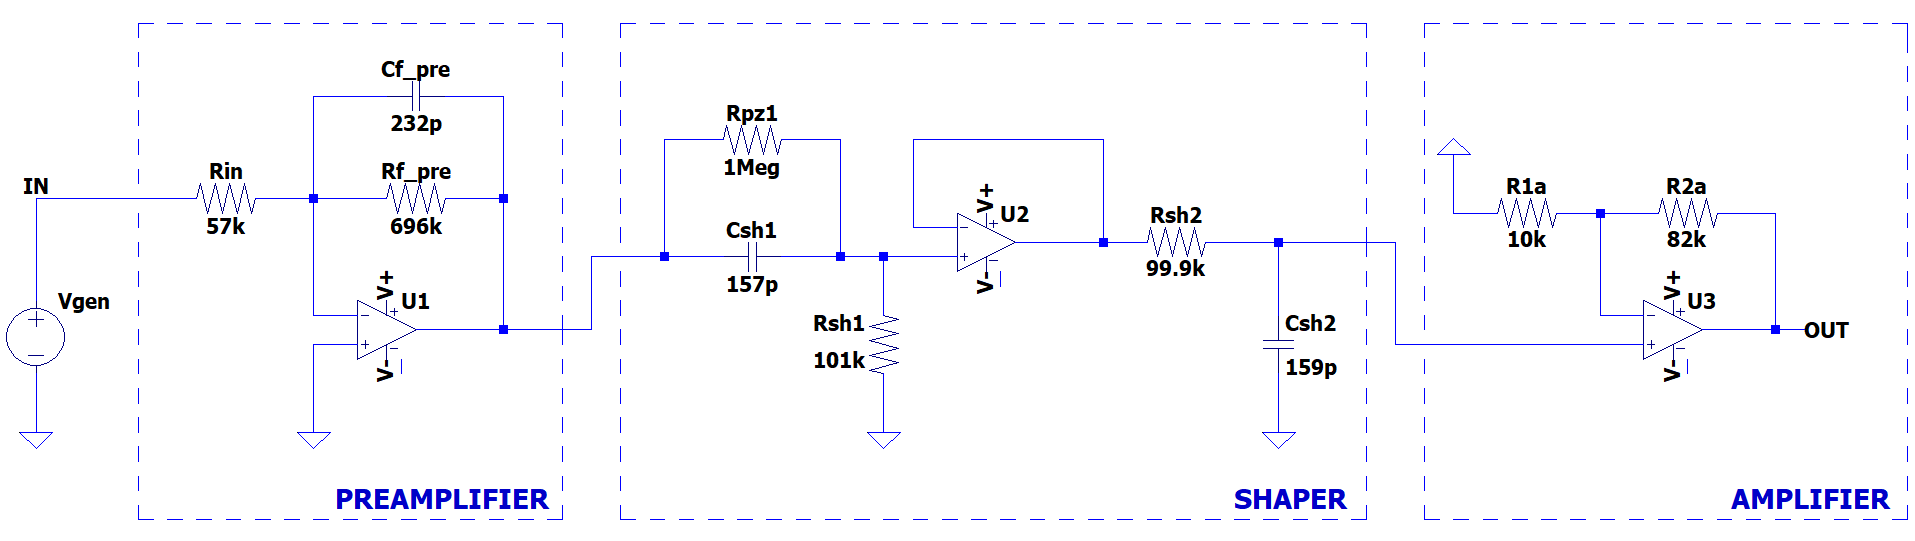
\includegraphics[width=0.9\linewidth]{../Simulations/catena_circuito.png}
	\caption{\small Schema a costanti concentrate della catena elettronica suddivisa nei tre moduli di interesse.}
	\label{i:circuito}
\end{figure}

%-------------------------------------------------------------------------------------------------------------------------------------------
%	PREAMPLIFICATORE
%-------------------------------------------------------------------------------------------------------------------------------------------

\section{Preamplificatore}\label{s:preamp} 

Il primo stadio della catena \textit{(preamplificatore)} si utilizza per migliorare il rapporto segnale/rumore, in modo
da trasferire un segnale più pulito all'elettronica di acquisizione. Si assembla in laboratorio un preamplificatore
\textit{charge sensitive}: come si può osservare in \autoref{i:circuito} il modulo consiste di un circuito integratore
e la tensione in uscita è quindi direttamente proporzionale alla carica in ingresso. Lo scopo di questa sezione,
dedicata al preamplificatore, è di studiare il segnale in uscita verificandone l'integrazione e la linearità rispetto
alla carica in ingresso, oltre alla risposta in frequenza del filtro passa basso ricercandone la frequenza di taglio.

%-------------------------------------------------------------------------------------------------------------------------------------------
%	CONFIGURAZIONE SPERIMENTALE
%-------------------------------------------------------------------------------------------------------------------------------------------

\subsection{Configurazione Sperimentale}\label{s:preamp_config}

Si comincia utilizzando il generatore per simulare i segnali del rivelatore, impostando sul CH1 un impulso quadrato di
frequenza $f_{\text{gen}} = 1 \,\si{k\Hz}$, tensione di riferimento $V_{\text{high}} = 0 \,\si{\volt}$, ampiezza
\textit{negativa} $V_{\text{low}} = -1 \,\si{\volt}$ e durata $T = 5 \,\si{\us}$ (cioè il tempo di raccolta del
segnale). Viene successivamente assemblato 

\begin{wraptable}{L}{0.5\textwidth}
	\small
	\centering
	\begin{tabular}{x{1.8cm} x{2.5cm} x{2cm} } \toprule[0.5px]\toprule[0.1px]	
		\multicolumn{3}{c}{Misure Dirette - Preamplificatore}\tn
		\midrule[0.1px]
		Label & Valore & F.S. \tn
		\addlinespace
		$R_{\text{in}}$ & $56.56 \pm 0.02\,\si{k\ohm}$ & $100\,\si{k\ohm}$ \tn
		$R_{\text{f}}$ & $696.1 \pm 0.3\,\si{k\ohm}$ & $1000\,\si{k\ohm}$ \tn
		$C_{\text{f}}$ & $232 \pm 9\,\si{p\farad}$ & $1000\,\si{p\farad}$ \tn
		\bottomrule[0.5px]		
	\end{tabular}
	\caption{\footnotesize Misure dirette delle componenti circuitali.}
	\label{t:direct_measures}
\end{wraptable}	

\noindent sulla breadboard il primo modulo in \autoref{i:circuito} utilizzando le componenti circuitali riportate in
\autoref{t:direct_measures}, misurate con il multimetro Metrix. Si utilizza poi un generatore di tensione continua con
$V_{\text{cc}}=+15\,\si{\volt}$ e $V_{\text{ee}}=-15\,\si{\volt}$ per alimentare l'operazionale. Si assume, inoltre, che
esso abbia un comportamento ideale, ovvero che il polo positivo ed il polo negativo si trovino allo stesso potenziale
(\textit{virtual short}). Il segnale in ingresso $V_{\text{in}}$ viene prelevato nel punto \textit{IN} evidenziato nello
schema mentre il segnale in uscita $V^{\text{pre}}_{\text{out}}$ dal preamplificatore viene prelevato al termine del
primo modulo, entrambi utilizzando sonde 10X. Concentrando l'attezione sul modulo di ingresso (generatore reale e
cablaggio), il sistema è un filtro passa basso con frequenza di taglio $f_{\text{t}}^{\text{in}}\approx 32 \,\si{\MHz}$
che risulta essere molto maggiore delle frequenze in gioco: risulta allora corretto assumere il modulo in ingresso del
tutto equivalente ad un generatore ideale, come rappresentato in \autoref{i:circuito}. Trattando ora il preamplificatore,
la funzione di trasferimento del circuito risulta essere 
\begin{align}\label{e:preamp_H}
	H(s) &= - \frac{ 1 }{ R_{\text{in}}\,C_{\text{f}} } \,\, \frac{1}{ s + \frac{ 1 }{ \tau_{\text{f}} } } & 
	&\text{con  } \,\, \tau_{\text{f}} = R_{\text{f}}\,C_{\text{f}} \equiv \tau^{\text{pre}}
\end{align}
\noindent Ricavando allora la risposta ad un segnale a gradino nell'approssimazione $T\ll\tau^{\text{pre}}$ si trova una
crescita lineare direttamente proporzionale alla carica in ingresso al preamplificatore per $0 < t < T$ e una
decrescita smorzata esponenzialmente per $t \gg T$:
\begin{align}\label{e:preamp_vout}
	V^{\text{pre}}_{\text{out}}(t) &= 
	\begin{cases} 
		-\frac{ Q_{\text{in}} (t) }{ C_{\text{f}} } & 0 < t < T \\
		-\frac{ Q_{\text{c}} }{ C_{\text{f}} } \, e^{ -\frac{ t }{ \tau^{\text{pre}} } } & t \gg T \\
	\end{cases}
	& 
	&\text{con} \,\,\, 
	\begin{cases} 
		Q_{\text{in}} (t) = I_{\text{in}}\,t = \frac{ V_{\text{in}} }{ R_{\text{in}} }\,t \\
		Q_{\text{c}} = I_{\text{in}}\,T = \frac{ V_{\text{in}} }{ R_{\text{in}} }\,T \\
	\end{cases}
\end{align}	
\noindent dove, appunto, $Q_{\text{in}} (t)$ corrisponde alla carica raccolta al tempo $t$ dal preamplificatore mentre
$Q_{\text{c}}$ rappresenta la carica \textit{totale} accumulata nel preamplificatore. Ci si aspetta allora che il
segnale in uscita $V^{\text{th}}_{\text{out}}$ visualizzato sull'oscilloscopio presenti una salita lineare, un valore di
tensione massimo corrispondente a $V_{\text{max}}^{\text{th}} = 0.388 \pm 0.017 \,\si{\volt}$ (misurando l'ampiezza del
segnale in ingresso $V_{\text{in}} = 1.02 \pm 0.02 \,\si{\volt}$), e successivamente una decrescita esponenziale di
tempo caratteristico $\tau^{\text{th}} = 161 \pm 6 \,\si{\us}$. Sperimentalmente, si misura un valore massimo
di tensione pari a $V^{\text{sper}}_{\text{max}} = 0.392 \pm 0.007 \,\si{\volt}$ e un tempo caratteristico di circa
$\tau^{\text{sper}} \approx 158 \,\si{\us}$, perfettamente in linea con le aspettative. Si vuole, in ogni caso,
approfondire lo studio della risposta del preamplificatore nelle sezioni successive. 

%-------------------------------------------------------------------------------------------------------------------------------------------
%	LINEARITA DEL PREAMP
%-------------------------------------------------------------------------------------------------------------------------------------------

\subsection{Linearità del Preamplificatore}\label{s:preamp_linearity}

Ci si propone ora di verificare la dipendenza lineare del segnale in uscita $V^{\text{pre}}_{\text{out}}$ dalla carica
in ingresso $Q_{\text{in}}$ come esposto in \autoref{e:preamp_vout}. Si fa variare dunque la durata $T$ del segnale
erogato dal generatore di funzioni da $2\,\si{\us}$ a $10\,\si{\us}$, in modo da modificare di volta in volta la
quantità di carica iniettata nel preamplificatore: per ogni $T$ viene calcolata la quantità di carica totale
$Q_{\text{c}}$ e viene misurato con l'oscilloscopio il valore massimo del segnale in uscita
$V^{\text{max}}_{\text{out}}$.  Ai valori di tensione misurati con l'oscilloscopio viene associato l'errore di
acquisizione comprendente sia il contributo di lettura sia il contributo sul guadagno verticale in quanto nel processo
di misura sono state utilizzate scale diverse, con la consapevolezza che quest'ultime portano ad una correlazioe almeno
parziale delle incertezze. Gli errori sulla carica $Q_{\text{c}}$, invece, sono totalmente correlati tra loro:
$V_{\text{in}}$ e $R_{\text{in}}$ sono, chiaramente, costanti e l'incertezza sulla carica è dunque semplicemente
l'incertezza sulla corrente in ingresso al preamplificatore $\sigma_{I_{\text{in}}}$ riscalata dal tempo $T$. Si assume,
ragionevolmente, che l'incertezza sulla durata $T$ del segnale sia trascurabile. Si rappresentano ora in
\autoref{i:preamp_linearity} le coppie $\{Q_{\text{c}},\,V^{\text{max}}_{\text{out}}\}$ interpolate da una retta: il
coefficiente angolare di quest'ultima corrisponde analiticamente all'inverso della capacità di feedback $C_{\text{f}}$.
Si vuole evidenziare che gli errori relativi su $V^{\text{pre}}_{\text{out}}$ e su $Q_{\text{c}}$ sono entrambi circa il
$2\%$ della misura: nell'effettuare la regressione si decide di trascurare l'incertezza sulla carica $Q_{\text{c}}$ (in
quanto totalmente correlata) e di aggiungere tale contributo successivamente nel calcolo dell'errore sulla capacità
$C_{\text{f}}$. La bontà del fit, l'andamento dei residui, l'errore a posteriori ed il confronto di
$C_{\text{f}}^{\text{fit}}$ con quanto misurato direttamente con il multimetro verranno presi in considerazione per
verificare la linearità del preamplificatore rispetto alla carica in ingresso.
\begin{figure}[H]
	\centering
	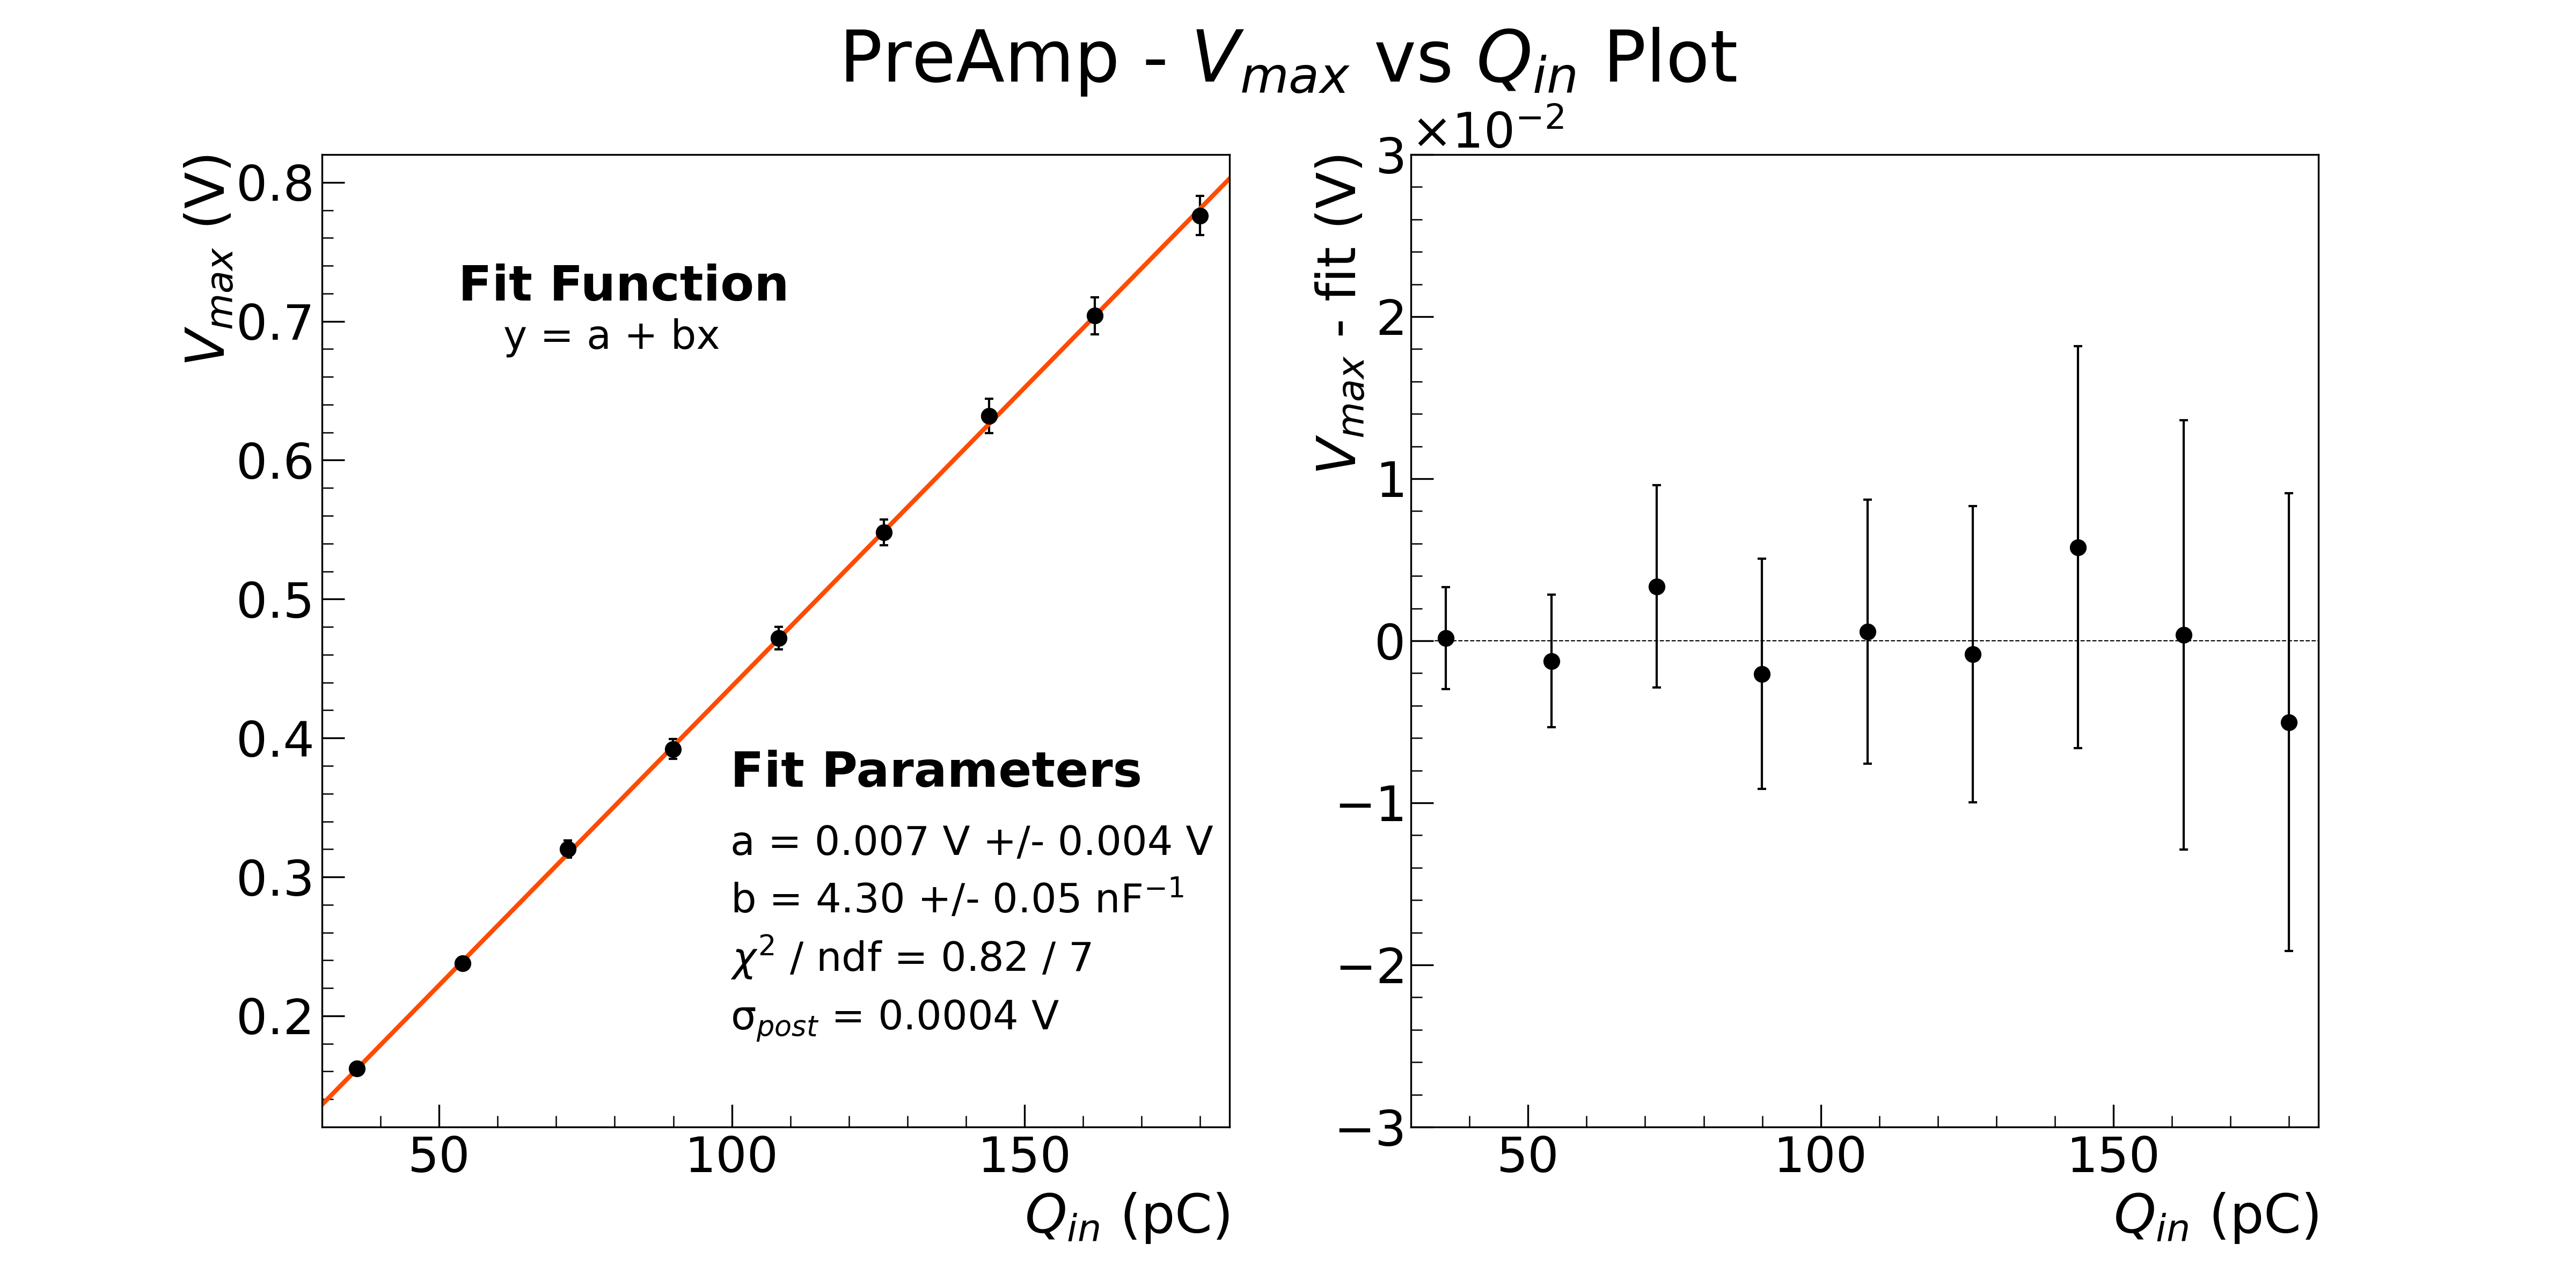
\includegraphics[width=0.9\linewidth]{../Plots/PreAmp/Vmax_Qin_lin_fit.png}
	\caption{\small Fit lineare del massimo di tensione in uscita contro la carica totale in ingresso.}
	\label{i:preamp_linearity}
\end{figure}
\noindent Si noti, inizialmente, come il $\chi^2$ della regressione sia notevolmente inferiore rispetto al suo valore di
aspettazione: essendo a conoscenza della parziale correlazione tra gli errori di scala dell'oscilloscopio ciò non
risulta essere sorprendente in quanto il fit non ne tiene ovviamente conto. Segue direttamente una sottostima
dell'errore sui parametri $a$ e $b$ della retta interpolante. Un piccolo (rispetto ai gradi di libertà) valore di
$\chi^2$ purtroppo non permette nè di confermare l'ipotesi di linearità nè di poterla rigettare. L'errore a posteriori,
invece, si trova essere dello stesso ordine di grandezza dell'errore associato alle tensioni più basse (i primi punti)
mentre diventa gradualmente un'ordine di grandezza inferiore rispetto all'incertezza associata alle tensioni maggiori.
Questo suggerisce una soddisfacente distribuzione dei punti attorno alla retta di regressione, che si traduce nel
grafico dei residui in un'ottimale distribuzione attorno allo zero. I residui, infatti, non presentano andamenti
patologici accentuati e lo zero risulta essere sempre ben compreso nelle barre d'errore. Concentrando ora l'attenzione
sui parametri della retta restituiti dal fit, si può notare come l'intercetta $a$ sia ben compatibile con zero,
evidenziando l'assenza di un eventuale offset sistematico o un errore di zero. Dal coefficiente angolare, invece, si
ricava la stima della capacità di feedback 
\begin{align}
	C_{\text{f}}^{\text{fit}}& = 0.232 \pm 0.007 \,\si{n\farad} 
	& 
	&\text{con} \,\,\,\, \sigma_{ C_{\text{f}}^{\text{fit}} } = 
	\sqrt
	{ 
		\left(
			\frac{1}{b^2}
		\right)^2
		\sigma_b^2 +
		2 \, \left(
			\frac{1}{b\,I}
		\right)^2
		\sigma_I^2
	}
\end{align}
\noindent dove, nel computo dell'errore, $\sigma_I$ rappresenta l'errore sulla corrente $I =
\frac{V_{\text{in}}}{R_{\text{in}}}$ che, nel fit, verrebbe riscalato dalla durata $T$ del segnale. La stima della
capacità di feedback risulta essere in ottima compatibilità ($\lambda = 0.05$) con quanto misurato con il multimetro
(\autoref{t:direct_measures}). Questo porta quindi ad un'ulteriore conferma della linearità del preamplificatore, che
risulta comportarsi conformemente alle aspettative teoriche. 

%-------------------------------------------------------------------------------------------------------------------------------------------
%	SMORZAMENTO ESPONENZIALE
%-------------------------------------------------------------------------------------------------------------------------------------------

\subsection{Forma d'Onda del segnale in uscita}\label{s:preamp_waveform}

In questa sezione si vuole analizzare il segnale in uscita dal preamplificatore $V^{\text{pre}}_{\text{out}}$:
sfruttando la stessa configurazione sperimentale presentata in \autoref{s:preamp_config} viene acquisita la forma d'onda
del segnale utilizzando la scheda Arduino Due. Inizialmente, si apportano le seguenti conversioni: dividendo il numero
di acquisizione per il sampling rate $S=0.955\,\text{Msps}$ si ottiene l'evoluzione temporale (in secondi) della forma
d'onda, mentre sfruttando la funzione di calibrazione in tensione $V= a  +  b \, \text{counts}$ (con $a=-0.637 \pm
0.010\,\si{\volt}$ e $b=0.828\pm0.007\,\si{mV/counts}$) si ottengono i valori in Volt delle misure acquisite in ADC
counts. A tali valori si associa l'errore per propagazione $\sigma_{V} = \sqrt{\sigma_a^2+\text{counts}^2\sigma_b^2}$:
si nota, tuttavia, che il contributo relativo a $\sigma_b$ è semplicemente riscalato per la misura in ADC counts
acquisita da arduino, ed è trattabile quindi come un errore di scala. In \autoref{i:preamp_waveform} è esposto quanto

\begin{wrapfigure}{R}{0.5\textwidth}
	\centering
	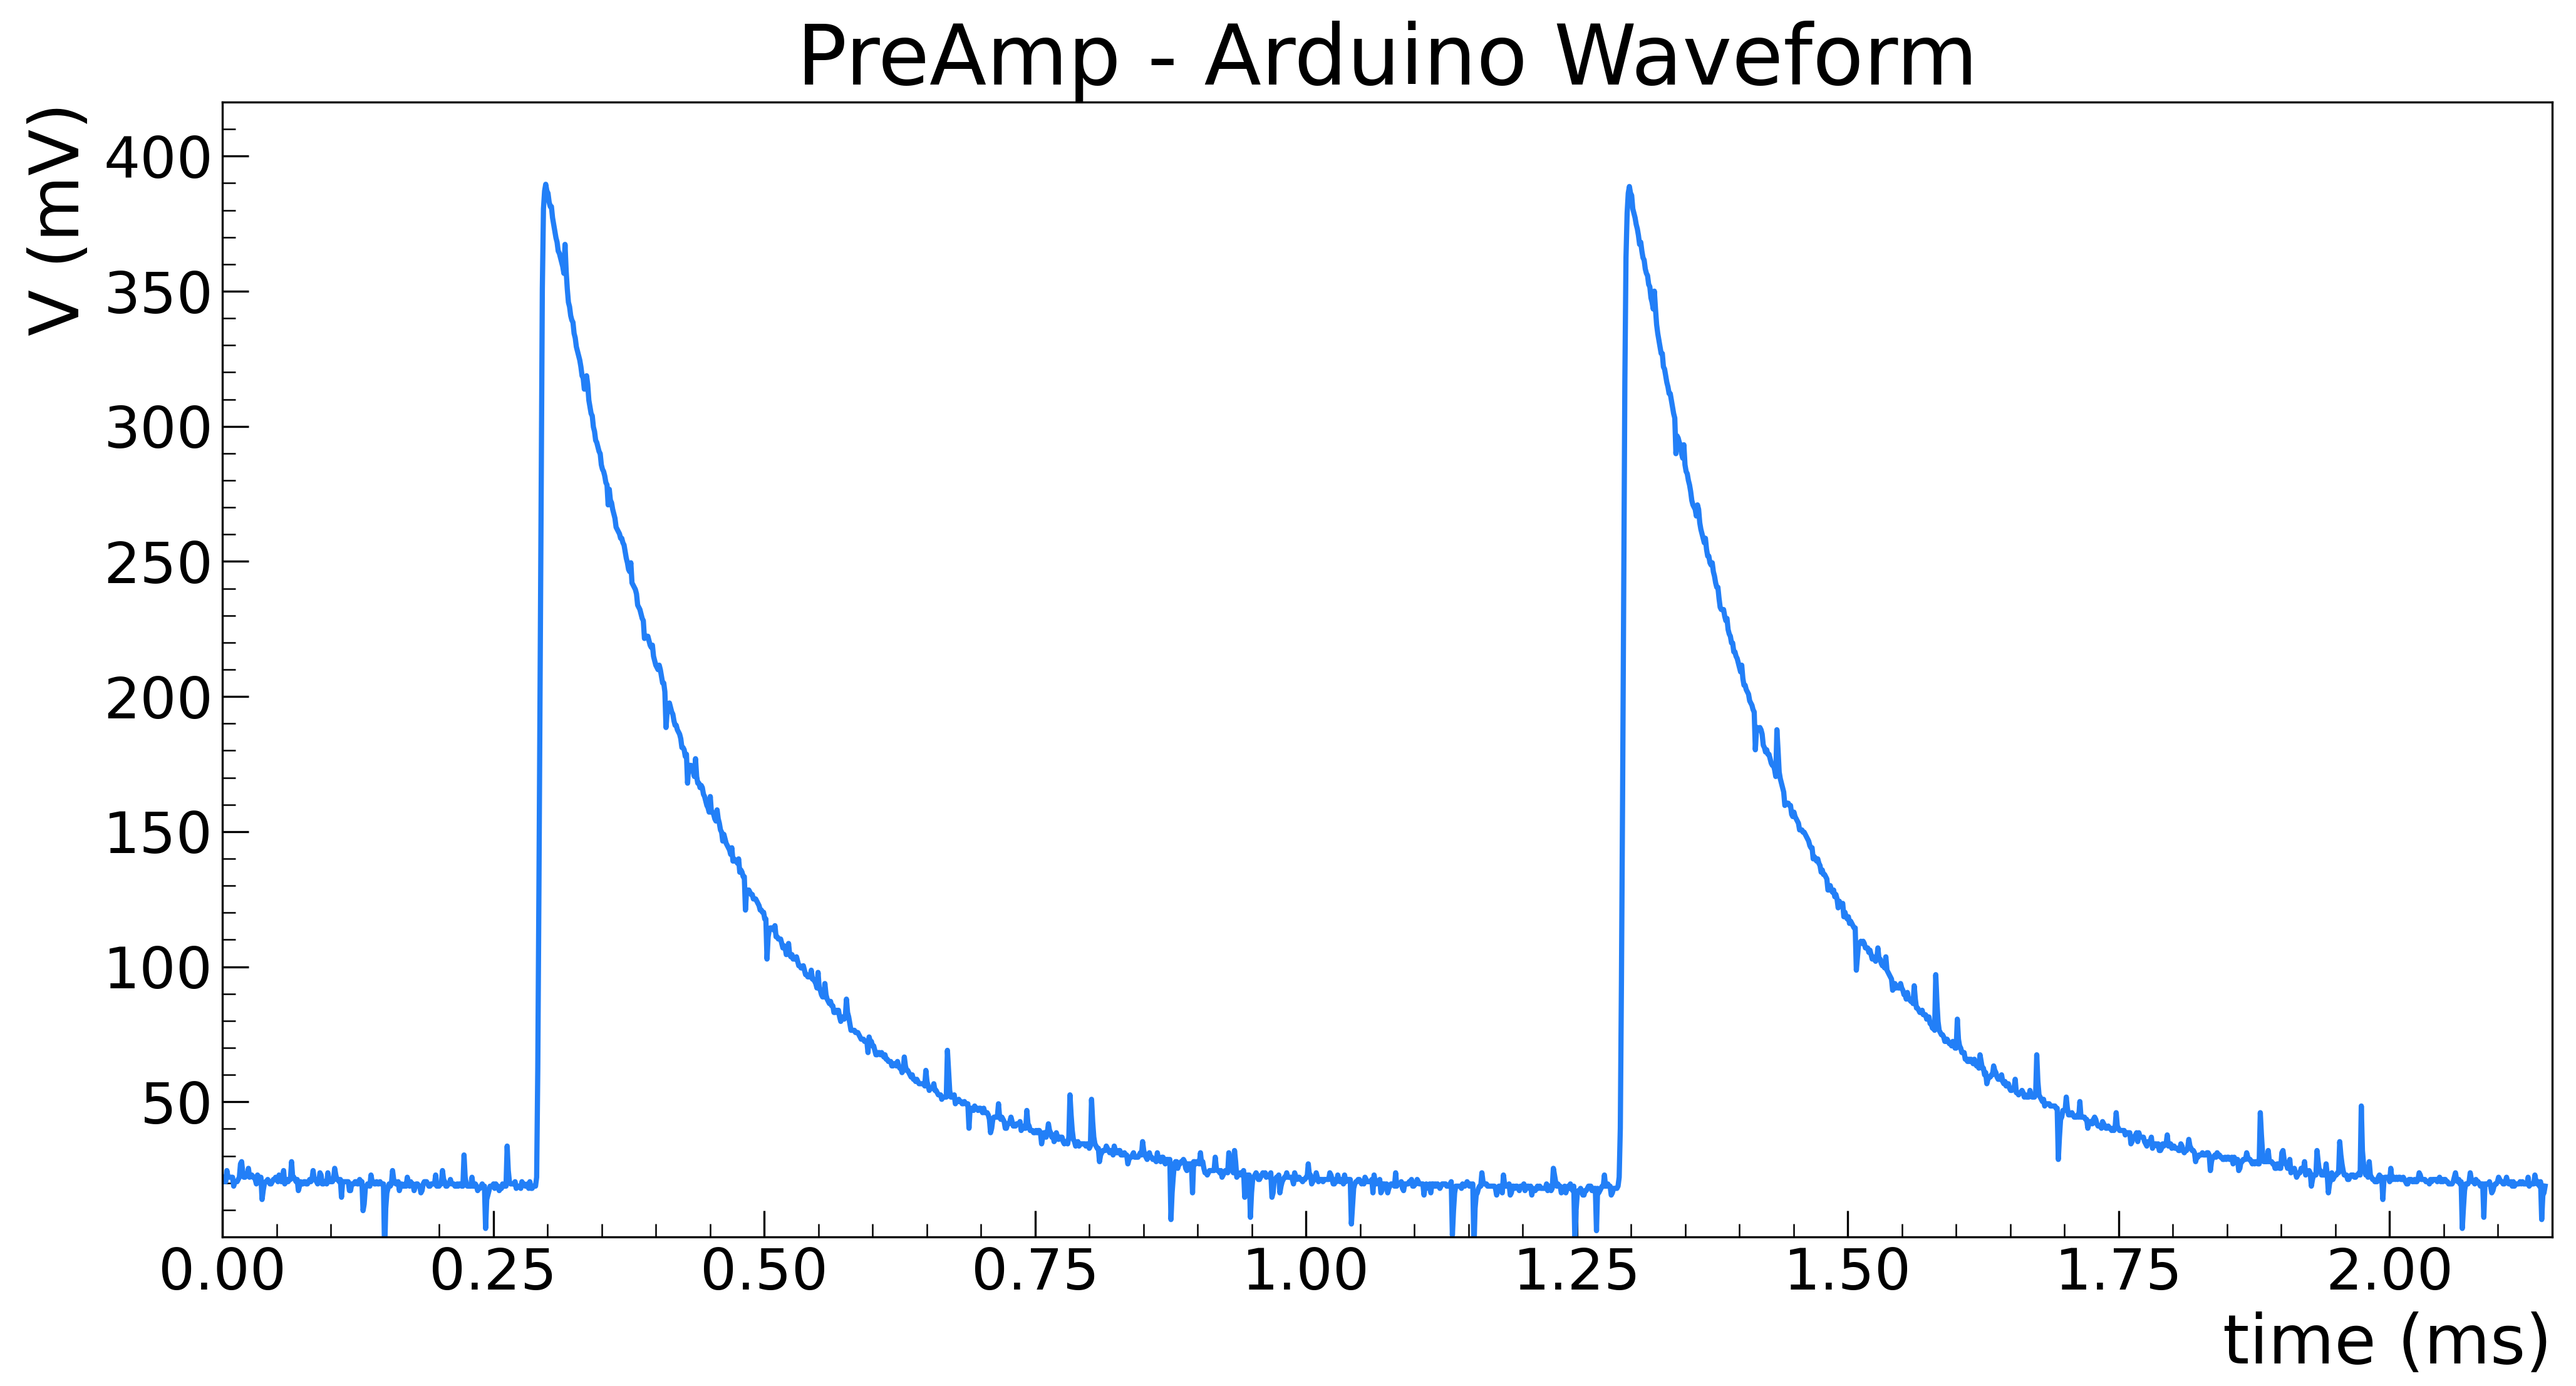
\includegraphics[width=0.5\textwidth]{../Plots/PreAmp/preamp_waveform.png}
	\caption{\small Segnale in uscita dal preamplificatore.}
	\label{i:preamp_waveform}
\end{wrapfigure}

\noindent  acquisito dalla scheda Arduino: si nota immediatamente come siano stati registrati due "eventi", o
meglio nel tempo di acquisizione impostato per Arduino il generatore di funzioni ha erogato due impulsi di tensione. Il
segnale registrato, inoltre, risulta essere leggermente rumoroso: per rendere l'analisi successiva meglio gestibile si
decide di sovrapporre i due picchi di tensione e di effettuarne una media. Osservando la \autoref{i:preamp_waveform}, si
può inoltre notare chiaramente la salita lineare del segnale e la descrescita esponenziale, come previsto in
\autoref{e:preamp_vout}. Il valore massimo di tensione acquisito con la scheda Arduino, inoltre, è in linea con le
aspettative e con quanto misurato sperimentalmente con l'oscilloscopio. Ci si concentra ora sulla stima del tempo
caratteristico $\tau^{\text{pre}}$: si vuole inizialmente effettuare un fit esponenziale del tipo $y = a +
b\,\text{exp}(-x/\tau)$. Successivamente, sfruttando i parametri $a$ e $b$ per normalizzare i dati, si vuole considerare
il logaritmo delle tensioni normalizzate ed effettuare una regressione lineare. Non è infatti possibile, per questioni
analitiche, considerare semplicemente il logaritmo delle tensioni $V$ ed aspettarsi un andamento lineare: si considera
invece il logaritmo delle tensioni normalizzate $\tilde{V} = (V-a)/b$ e l'errore su $\tilde{V}$ è dato per propagazione.
In questo modo, quindi, i dati si distribuiscono secondo $\log(\tilde{V})= -\frac{t}{\tau}$. Nell'effettuare il fit
esponenziale si decide di tenere conto dell'errore di scala dato dalla calibrazione della scheda Arduino, mentre per
quanto riguarda la regressione lineare si sceglie di non considerarlo in quanto, computando il logaritmo delle
tensioni, tale contributo viene interamente scaricato nell'offset della retta del fit. 
\begin{figure}[H]
	\centering
	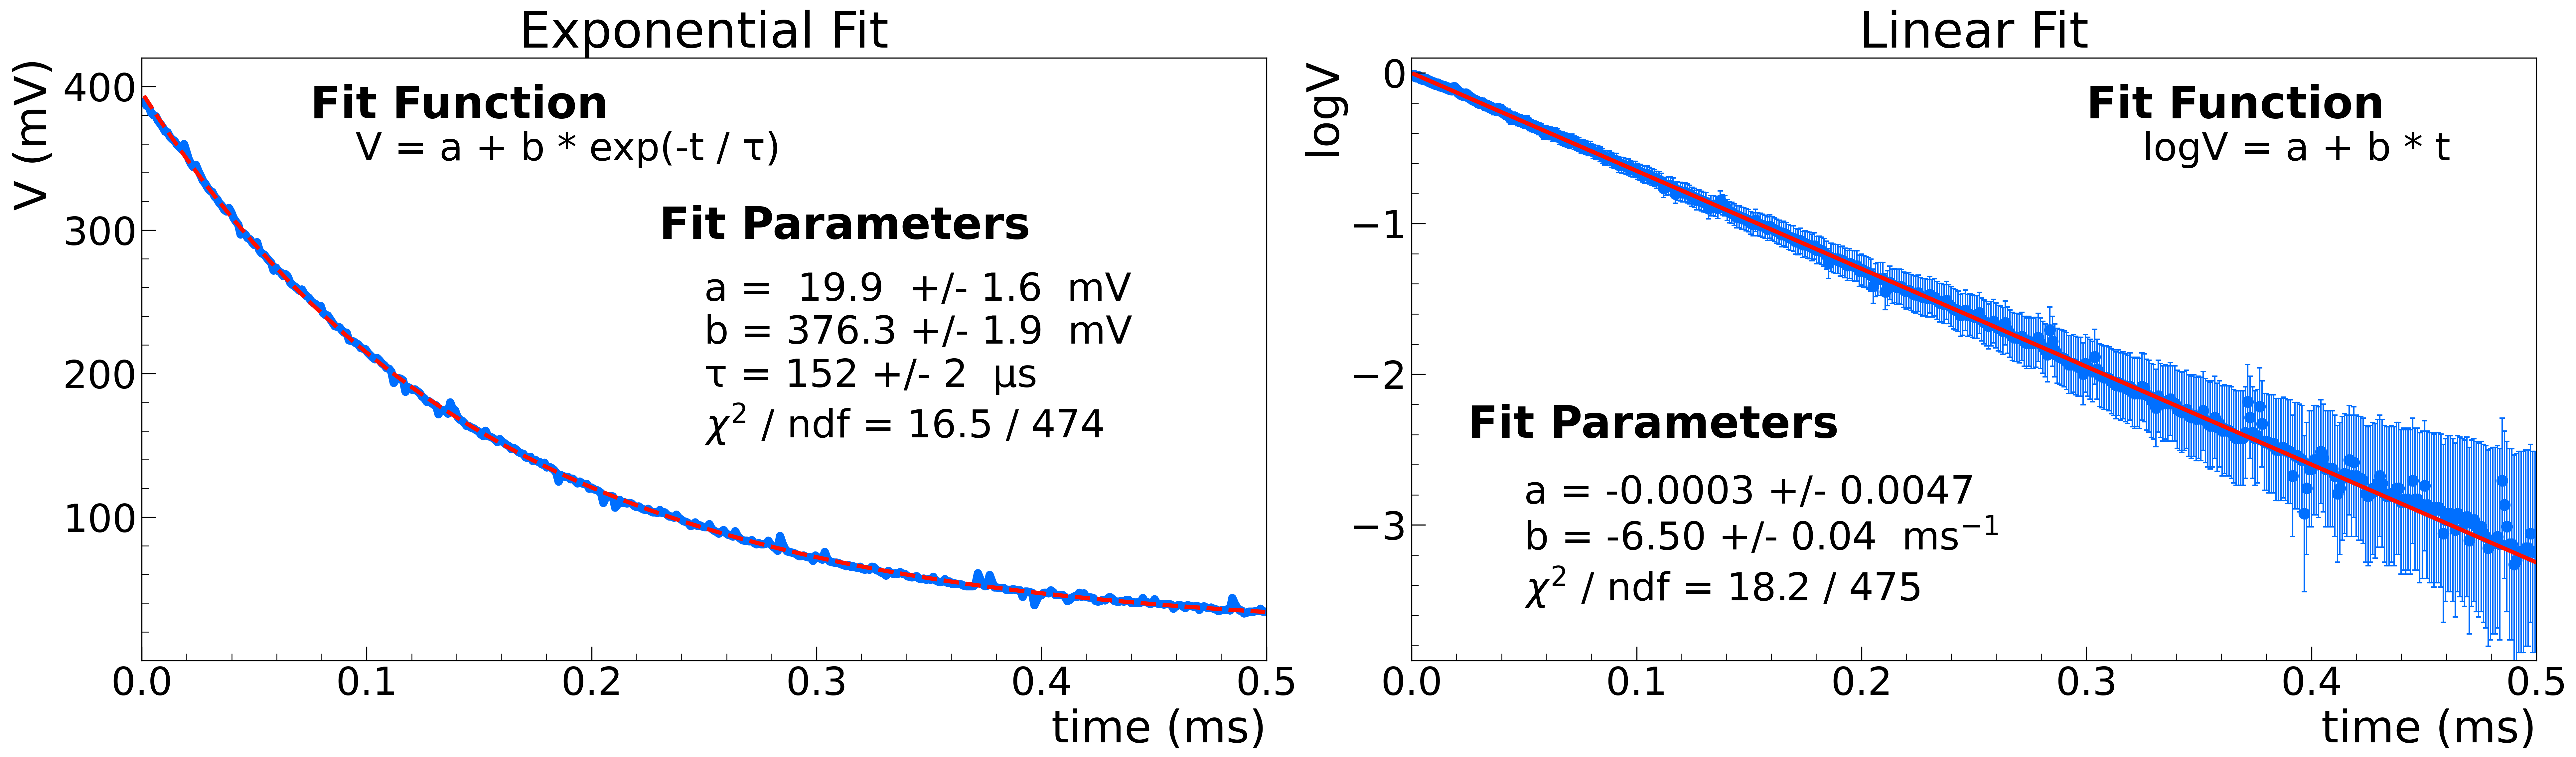
\includegraphics[width=\linewidth]{../Plots/PreAmp/preamp_arduino_fit.png}
	\caption{\small A sinistra: fit esponenziale dello smorzamento del segnale in uscita. 
					A destra: fit lineare del logaritmo del segnale in uscita normalizzato.}
	\label{i:preamp_arduino_fit}
\end{figure}
\noindent Osservando rapidamente il grafico a sinistra, si nota come il segnale segua in modo ottimale la funzione
esponenziale: la stima del tempo caratteristico $\tau^{\text{exp}}$, inoltre, risulta essere sufficientemente
compatibile con la stima teorica $\tau^{\text{th}} = 161 \pm 6 \,\si{\us}$ ($\lambda = 1.4$). Come stima del tempo
caratteristico, in ogni caso, si preferisce quanto trovato dalla regressione lineare: tale metodo, infatti, è
complessivamente più robusto, più preciso e fornisce una stima migliore sugli errori dei parametri. Dal grafico a
destra, quindi, si nota chiaramente come computare il logaritmo delle tensioni $\tilde{V}$ porti a considerare più
"pesanti" (barre d'errore più piccole) i punti a monte della discesa esponenziale e a dare conseguentemente meno peso ai
punti di coda. Questi ultimi, eccessivamente prossimi allo zero, non vengono considerati dato che la propagazione
dell'errore su di essi porta ad un contributo decisamente troppo grande ed il fit non ne è praticamente influenzato. Il
$\chi^2$, molto minore del suo valore di aspettazione, indica una probabile sovrastima dell'errore: le misure in cima
alla discesa si distribuiscono estremamente fedelmente attorno alla retta, compatibilmente con il loro errore, mentre le
misure verso la coda risultano discostarsi più sensibilmente dal fit. Tuttavia, sembra che l'incremento dell'errore su
queste ultime sia eccessivo, e che queste si distribuiscano attorno alla retta più fedelmente di quanto ci si aspetta
dalle barre d'errore. Calcolando ora il tempo caratteristico si trova $\tau^{\text{lin}}= -1/b = 153.9 \pm 1.0
\,\si{\us}$: questo presenta infine una compatibilità $\lambda = 1.2$ con  la stima teorica $\tau^{\text{th}}$.


%-------------------------------------------------------------------------------------------------------------------------------------------
%	THEBODE
%-------------------------------------------------------------------------------------------------------------------------------------------

\subsection{Grafico di Bode}\label{s:preamp_bode}

Si vuole ora studiare la risposta in frequenza del preamplificatore: si modificano le impostazioni del generatore in
modo da erogare un'onda sinusoidale di ampiezza $1\,\si{\volt}$ e frequenza $f_{\text{gen}}$ variabile da $10\,\si{\Hz}$
a $1\,\si{\MHz}$. Per quanto riportato in \autoref{e:preamp_H}, ci si aspetta un comportamento da filtro passa basso
avente frequenza di taglio
\begin{align}\label{e:preamp_ft_th}
	f_{\text{t}}&=\frac{1}{2\pi R_{\text{f}}C_{\text{f}}}= 0.99 \pm 0.04 \,\si{k\Hz} & 
	\text{con\,\,\,\,}\sigma_{f_{\text{t}}}&
	=\frac{1}{2\pi}\sqrt{	\left(\frac{1}{C_{\text{f}}R_{\text{f}}^2}\right)^2\sigma_{R_{\text{f}}}^2	+
	 \left(\frac{1}{C_{\text{f}}^2R_{\text{f}}}\right)^2\sigma_{C_{\text{f}}}^2   }																		
\end{align}
\noindent Si intende ora rappresentare le misure acquisite sperimentalmente attraverso un grafico di Bode. Viene
acquisita allora l'ampiezza del segnale sia in ingresso sia in uscita utilizzando l'oscilloscopio e viene calcolata la
funzione di trasferimento $H$, alla quale viene associata un'incertezza $\sigma_{H}$ data da
\begin{align}\label{e:preamp_H_err}
	H&=\frac{V_{\text{out}}}{V_{\text{in}}} & 
	\sigma_{H}&= H \sqrt{	
						\left(	\frac{	\sigma_{\text{L}}\times V_{\text{in}}/\text{div}	}{	V_{\text{in}}	}	\right)^2	 + 
						\left(	\frac{	\sigma_{\text{L}}\times V_{\text{out}}/\text{div}	}{	V_{\text{out}}	}	\right)^2 }
\end{align}
\noindent dove $\sigma_{\text{L}}=0.04$ rappresenta l'incertezza di lettura associata all'oscilloscopio mentre i termini
$V_{\text{in}}/\text{div}$ e $V_{\text{out}}/\text{div}$ corrispondono al numero di Volt per divisione per il canale di
acquisizione rispettivamente del segnale in ingresso e del segnale in uscita. L'incertezza di guadagno associata
all'oscilloscopio non viene invece considerata in quanto, dovendo successivamente prendere il logaritmo
$\text{log}_{10}H$ della funzione di trasferimento, tale contributo viene scaricato interamente nell'intercetta delle
interpolazioni volte a caratterizzare l'andamento delle misure. Si assume infine trascurabile l'incertezza sulla
frequenza dell'onda erogata dal generatore. Si rappresenta allora in \autoref{i:preamp_thebode} il grafico di Bode delle
misure acquisite assieme ai punti ottenuti attraverso una simulazione Spice della risposta del circuito.
\begin{figure}[H]
	\centering
	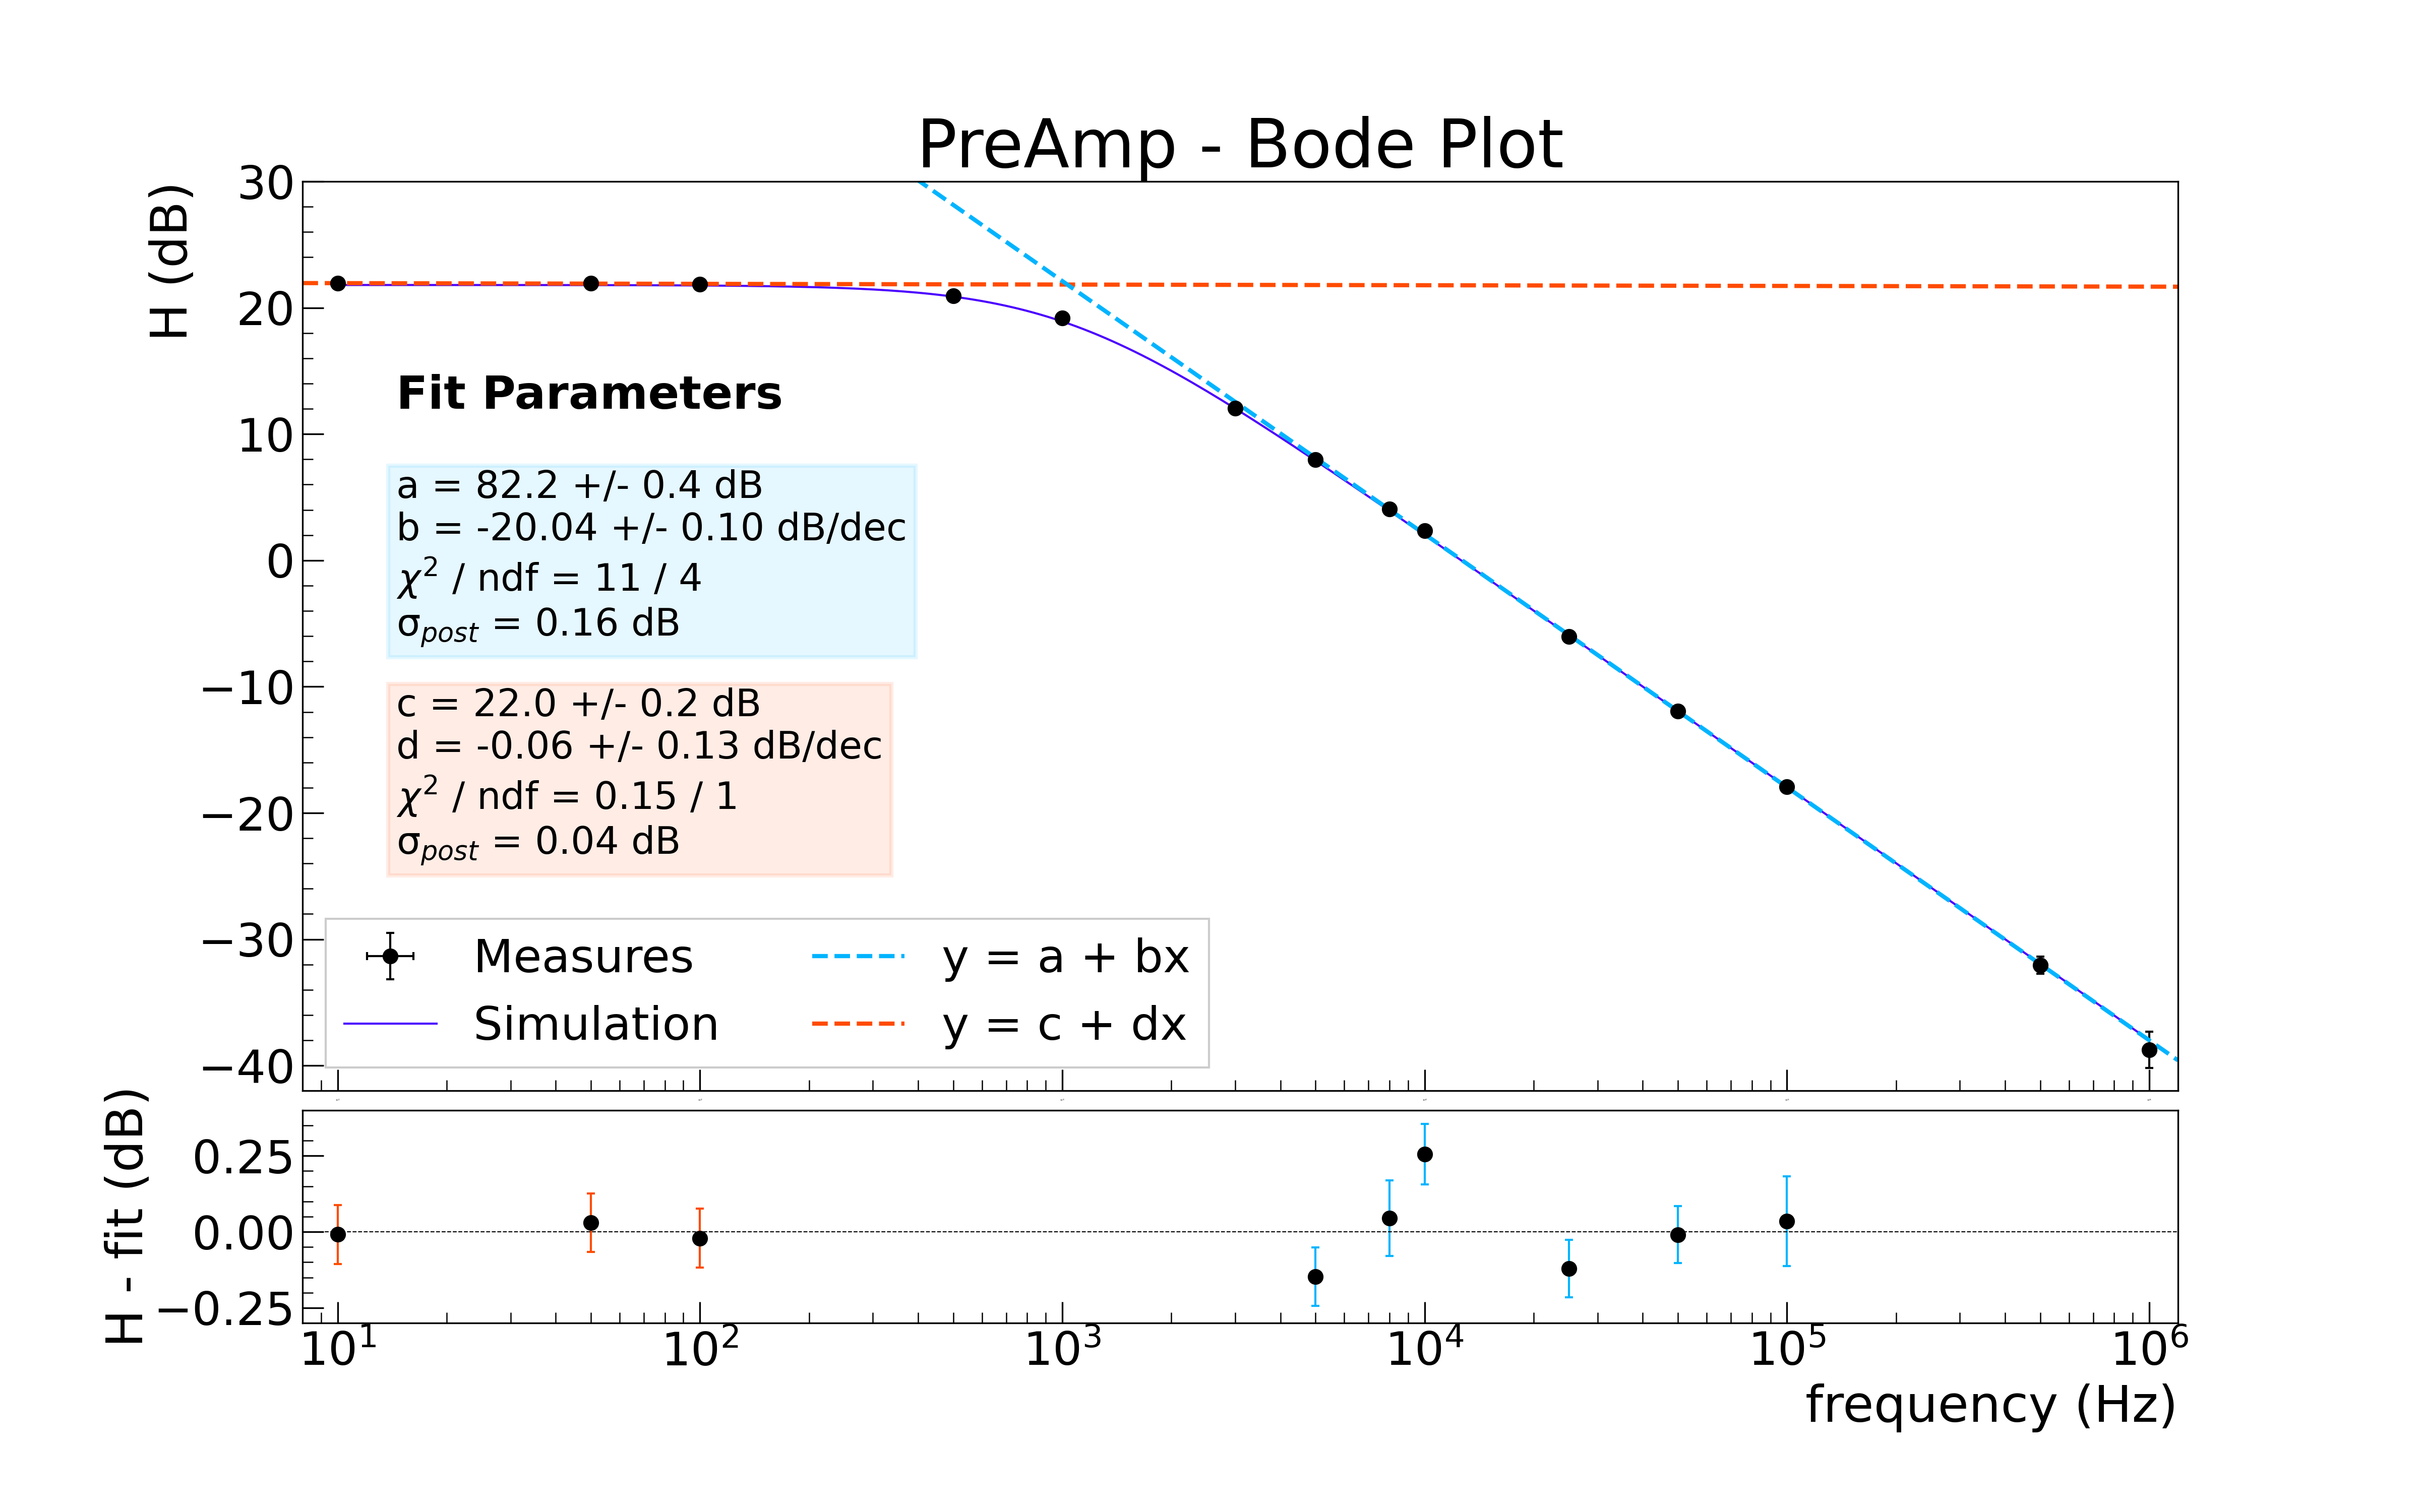
\includegraphics[width=0.9\linewidth]{../Plots/PreAmp/bode_plot.png}
	\caption{\small Grafico di Bode delle misure sperimentali e dei dati simulati.}
	\label{i:preamp_thebode}
\end{figure}
\noindent Confrontando inizialmente le misure sperimentali con la simulazione Spice, si nota un ottimo accordo in tutto
lo spettro di frequenze. Questo è chiaramente indice di una risposta in frequenza del circuito compatibile con le
aspettative: il comportamento del filtro, infatti, è evidentemente un passa basso. A basse frequenze, la funzione di
trasferimento è pressochè costante a $22\,\si{dB}$ (retta in \textit{arancione}), mentre per frequenze crescenti la
funzione di trasferimento decresce linearmente con coefficiente angolare conforme all'aspettativa dei
$-20\,\si{dB/dec}$. L'ascissa del punto di intersezione tra le due rette di regressione fornisce una stima della
frequenza di taglio del circuito $f_{\text{t}} = 1.03 \pm 0.03 \,\si{\kHz}$, compatibile in modo soddisfacente ($\lambda
= 0.9$) con la frequenza di taglio teorica esposta in \autoref{e:preamp_ft_th}. Si vuole sottolineare che nel computo
dell'errore su $f_{\text{t}}$ è stata presa in considerazione la convarianza tra parametri appartenenti allo stesso fit.
Osservando infine che la formula analitca frequenza di taglio $f_{\text{t}}$ riportata in \autoref{e:preamp_ft_th}
contiene il termine $R_{\text{f}} \, C_{\text{f}}=\tau^{\text{pre}}$, si vuole valutare l'accordo tra la frequenza di
taglio ottenuta dal grafico di Bode e la frequenza di taglio teorica, utilizzando però
$\tau^{\text{pre}}=\tau^{\text{lin}}$ ricavato nella sezione precedente. Si ottiene dunque una frequenza di taglio
$f_{\text{t}}^{\text{lin}} = 1.034 \pm 0.007 \,\si{\kHz}$ ed è in eccellente compatibilità con quanto appena stimato
($\lambda = 0.13$). Da questo notevole accordo si deduce l'assenza di possibili sistematicità di metodo, sia nella stima
del tempo caratteristico attraverso il fit lineare in \autoref{i:preamp_arduino_fit}, sia nella stima della frequenza di
taglio analizzando il grafico di Bode. 

%-------------------------------------------------------------------------------------------------------------------------------------------
%	SHAPER
%-------------------------------------------------------------------------------------------------------------------------------------------

\section{Shaper CR-RC}\label{s:shaper} 

Il secondo stadio della catena (\textit{shaper}) si utilizza per modificare la
forma del segnale in uscita dal preamplificatore. Si vuole, in particolare, accorciare il tempo di discesa al fine di
evitare un possibile \textit{signal pile up} nel caso di un'elevata frequenza di acquisizione. In tale situazione,
infatti, il segnale di un acquisizione successiva si sovrapporrebbe (almeno parzialmente) a quello dell'acquisizione
precedente, rendendo estremamente più complicato estrarre le corrette informazioni dalle due acquisizioni. È inoltre
importante che lo shaper preservi l'informazione sulla carica in ingresso, in quanto questa risulta essere il modello
utilizzando nell'esperienza per simulare l'evento rivelato dal detector. Nelle sezioni successive, quindi, si vuole
verificare che il segnale in uscita sia direttamente proporzionale al segnale in ingresso e che la durata del segnale in
uscita sia ridotta rispetto allo smorzamento esponenziale della tensione dovuto al preamplificatore. 

%-------------------------------------------------------------------------------------------------------------------------------------------
%	CONFIGURAZIONE SPERIMENTALE IDEALE
%-------------------------------------------------------------------------------------------------------------------------------------------

\subsection{Configurazione Sperimentale Ideale}\label{s:shaper_config_ideale}

Si comincia assemblando sulla breadboard il secondo modulo rappresentato in \autoref{i:circuito} utilizzando le
resistenze e capacità riportate in \autoref{t:shaper_direct_measures}. Si evidenzia che per la prima fase di analisi non
viene montata la resistenza $R_{\text{pz}}$: la compensazione di \textit{pole zero} verrà trattata in seguito.
Inizialmente, allora,

\begin{wraptable}{L}{0.5\textwidth}
	\small
	\centering
	\begin{tabular}{x{1.8cm} x{2.5cm} x{2cm} } \toprule[0.5px]\toprule[0.1px]	
		\multicolumn{3}{c}{Misure Dirette - Shaper}\tn
		\midrule[0.1px]
		Label & Valore & F.S. \tn
		\addlinespace
		$R_{1}$ & $100.99 \pm 0.06\,\si{k\ohm}$ & $1000\,\si{k\ohm}$ \tn
		$R_{2}$ & $99.93  \pm 0.06\,\si{k\ohm}$ & $1000\,\si{k\ohm}$ \tn
		$C_{1}$ & $157    \pm 9 \,\si{n\farad}$ & $1000\,\si{p\farad}$ \tn
		$C_{2}$ & $159    \pm 9 \,\si{n\farad}$ & $1000\,\si{p\farad}$ \tn
		\bottomrule[0.5px]		
	\end{tabular}
	\caption{\footnotesize Misure dirette delle componenti circuitali.}
	\label{t:shaper_direct_measures}
\end{wraptable}	

\noindent  si vuole studiare il comportamento dello shaper in risposta ad un segnale \textit{ideale}, tale da avere una
salita (quasi) istantanea e da rimanere costante al valore massimo. Un tale segnale viene simulato facendo erogare al
generatore di funzioni un'onda quadra a bassa frequenza ($100\,\si{\Hz}$) di tensioni $V_{\text{low}} = 0\,\si{\volt}$ e
$V_{\text{high}} = 1\,\si{\volt}$. Prima di trattare analiticamente il circuito, calcolando la funzione di trasferimento
e la risposta ad un segnale a gradino, si vuole far notare che la presenza del \textit{buffer} tra il modulo CR ed il
modulo RC permette di fattorizzare la funzione di trasferimento complessiva del circuito $H(s) = H_{\text{CR}} \,
H_{\text{RC}}$, dove $H_{\text{CR}}$ e $H_{\text{RC}}$ sono semplicemente le funzioni di trasferimento di un circuito RC
rispettivamente in configurazione passa alto e passa basso. In questo modo quindi il calcolo della funzione di
trasferimento si semplifica notevolmente ed il comportamento del filtro risulta essere più prevedibile. Inoltre, per la
trattazione analitica del circuito e della sua risposta si considera l'approssimazione $R_1 \, C_1 \equiv
\tau^{\text{sh}}_1 \approx \tau^{\text{sh}}_2 \equiv R_2 \, C_2$, ragionevole in quanto si ha $\tau^{\text{sh}}_1 =
15.86 \pm 0.91 \,\si{\us}$ e $\tau^{\text{sh}}_2 = 15.89 \pm 0.90 \,\si{\us}$ (si mostrano due cifre decimali
esclusivamente per evidenziare la sottile differenza tra i due valori). Come tempo caratteristico dello shaper si
considera allora la media pesata $\tau^{\text{sh}} = 15.9 \pm 0.6 \,\si{\us}$. In questa approssimazione, la funzione di
trasferimento del circuito risulta essere
\begin{align}\label{e:shaper_H}
	H(s) &= \frac{ 1 }{ \tau^{ \text{sh} } }  \,  \frac{ s }{ \left( s + \frac{ 1 }{ \tau^{ \text{sh} } } \right)^2}  &
	&\text{con} \,\,\,\, \tau^{\text{sh}}= 15.9 \pm 0.6 \,\si{\us}
\end{align}
\noindent Si nota allora come la funzione di trasferimento presenti uno zero nell'origine ed un polo doppio legato \newpage  

\noindent al tempo caratteristico $\tau^{\text{sh}}$. Il grafico di Bode del comportamento in frequenza atteso presenta
dunque una salita lineare di $20\,\si{dB/dec}$ fino al raggiungimento del polo $f_{\text{polo}}= \frac{1}{2\pi\tau^{
\text{sh} }}$ e successivamente una discesa lineare di $-20\,\si{dB/dec}$. Il comportamento dunque è tipico di un filtro
passa banda, la cui banda passante è influenzata dallo \textit{shaping time} $\tau^{ \text{sh} }$. Concentrando ora
l'attenzione sulla risposta dello shaper ad un segnale in ingresso ideale, ci si aspetta in uscita una tensione data da
\begin{equation}
	V_{\text{out}}(t)=\frac{V_{\text{in}}}{\tau^{ \text{sh} }} \, t \, e^{-\frac{t}{ \tau^{ \text{sh} } }}
\end{equation}
\noindent che presenta un massimo $V_{\text{out}}^{\text{max}}= V_{\text{in}}/e$ direttamente proporzionale al segnale
in ingresso, che quindi preserva l'informazione sulla carica raccolta dal preamplificatore. Inoltre, tale massimo viene
assunto 

\begin{wrapfigure}{R}{0.5\textwidth}
	\centering
	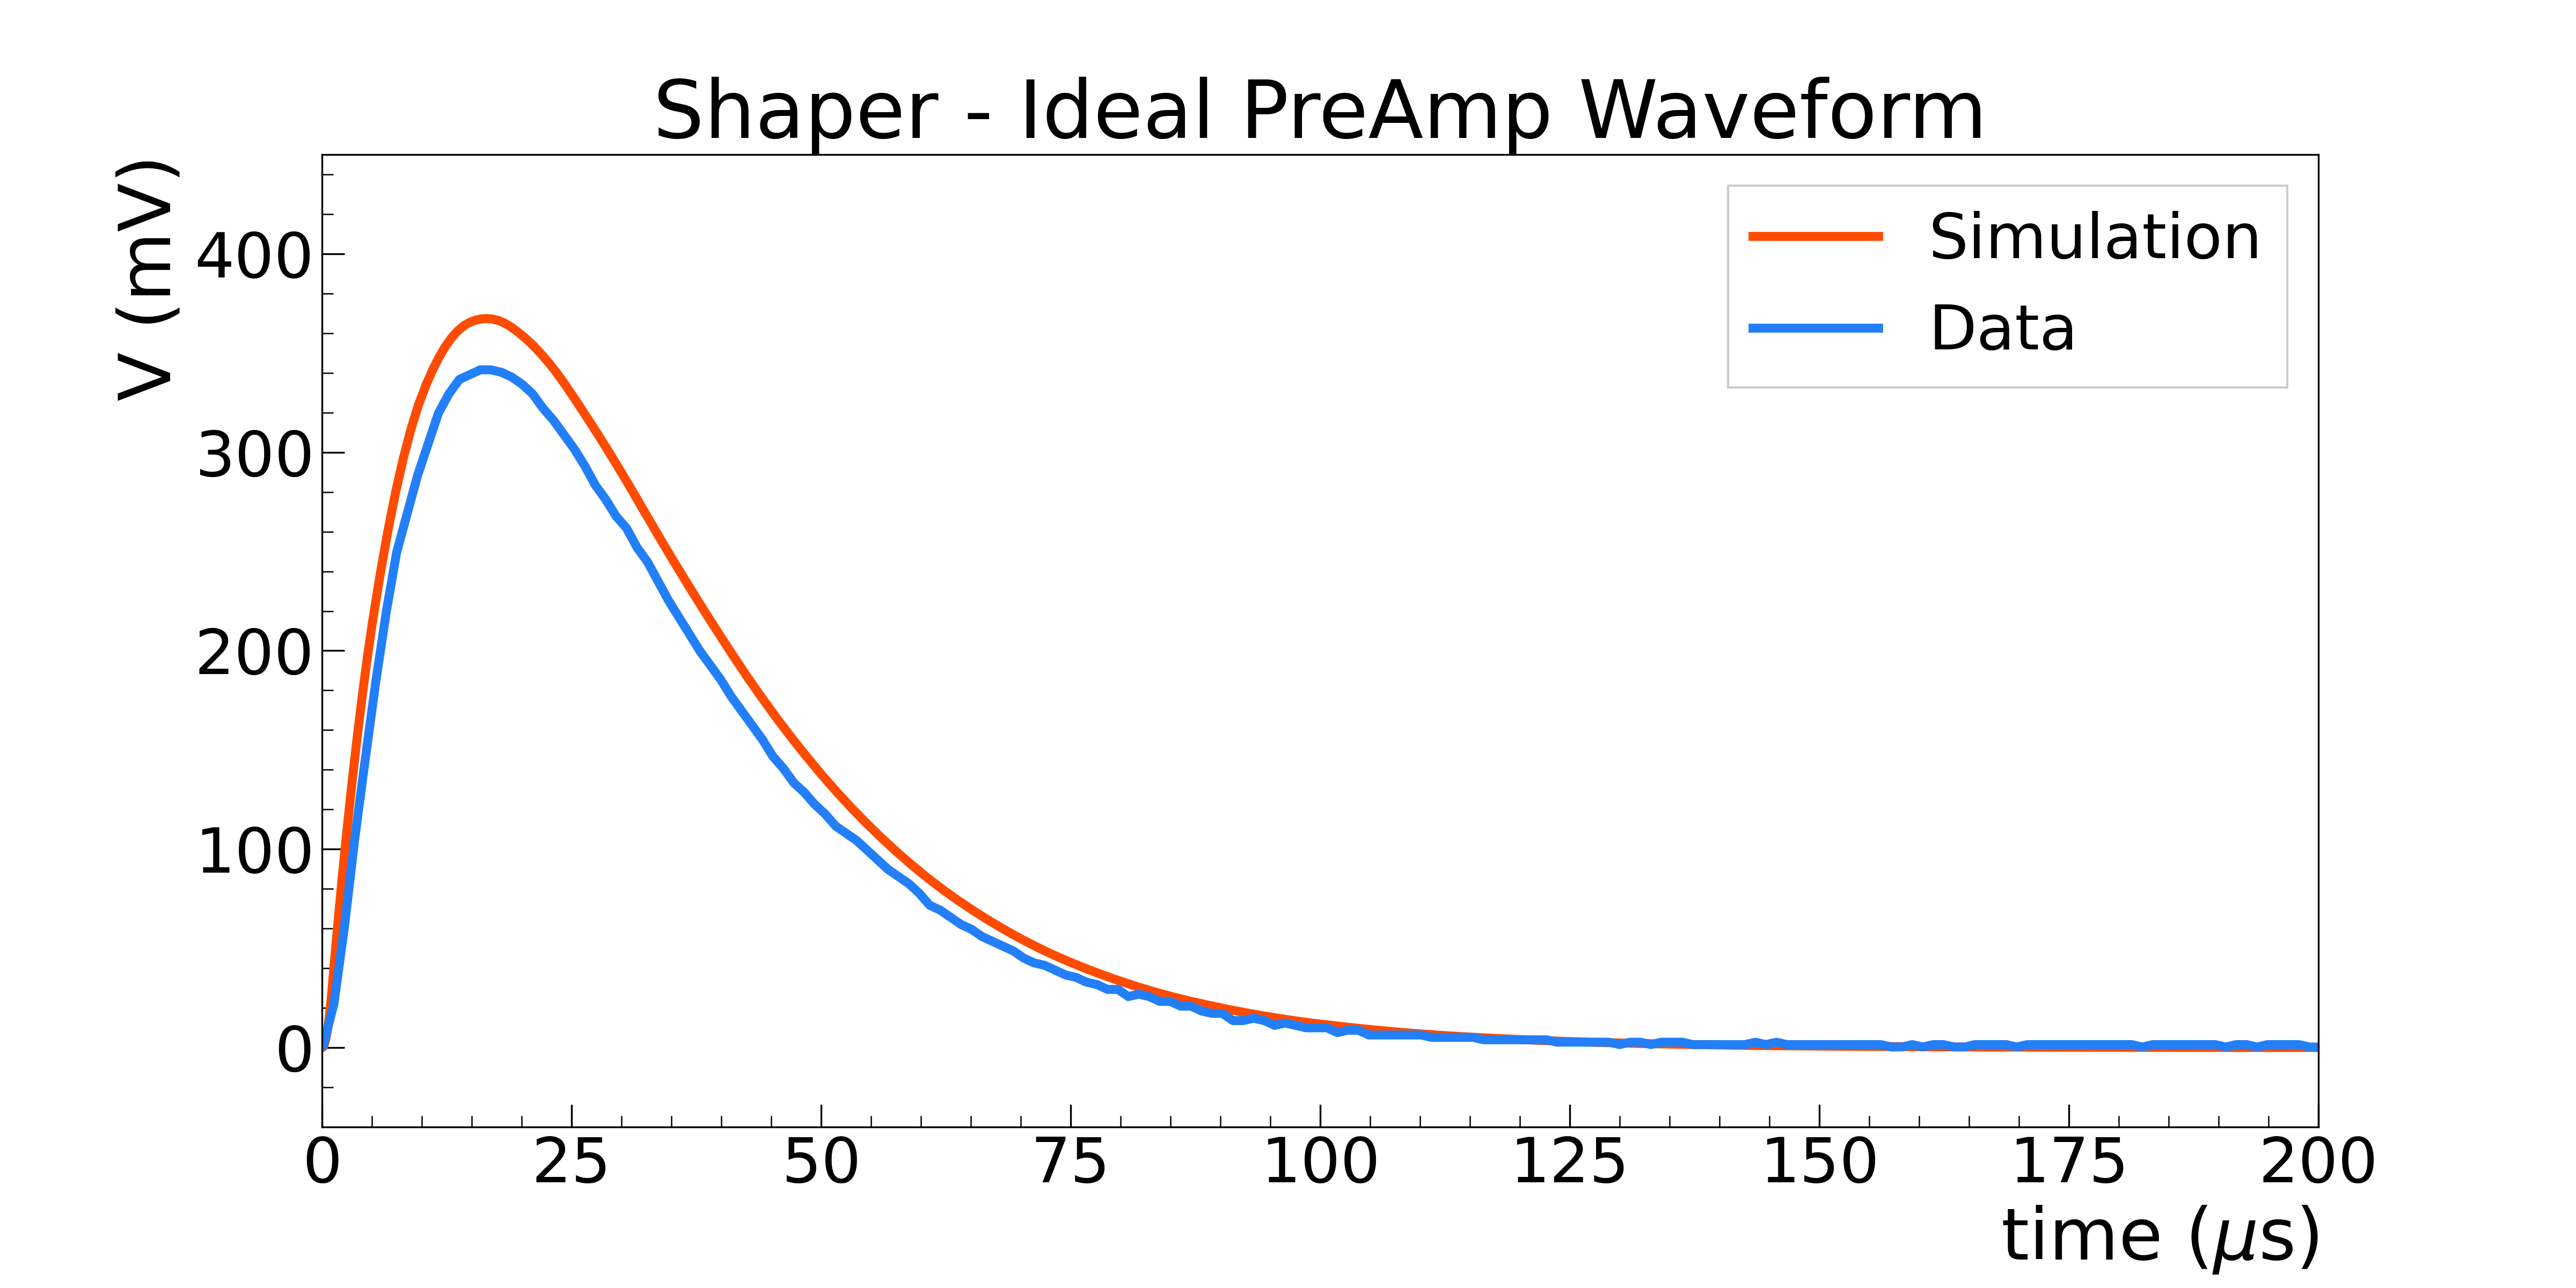
\includegraphics[width=0.5\textwidth]{../Plots/Shaper/shaper_ideal.png}
	\caption{\small Segnale in uscita dallo shaper.}
	\label{i:shaper_ideal}
\end{wrapfigure}

\noindent ad un tempo $t^{\text{max}} = \tau^{\text{sh}}$: lo \textit{shaping time}, quindi, determina approssimativamente
la durata del segnale in uscita dallo shaper. Si noti che $\tau^{\text{sh}}$ è un ordine di grandezza inferiore rispetto
al tempo caratteristico $\tau^{\text{pre}}$: da questo si deduce quindi che la durata del segnale viene notevolmente
ridotta grazie all'azione dello shaper, come anticipato in \autoref{s:shaper}. Avendo misurato con l'oscilloscopio il
segnale in ingresso, ci si aspetta allora un segnale massimo in uscita $V_{\text{th}}^{\text{max}}= 0.372 \pm
0.006\,\si{\volt}$, mentre sperimentalmente si misura $V_{\text{sper}}^{\text{max}}= 0.342 \pm 0.006\,\si{\volt}$:
quest'ultimo si discosta del $7.9\%$ rispetto al primo. Questa incongruenza tra aspettativa teorica e misura
sperimentale si attribuisce principalmente alle componenti circuitali ed alle sistematiche presenti nel circuito stesso.
Il valore massimo $V_{\text{sper}}^{\text{max}}$ viene invece assunto ad un tempo conforme allo \textit{shaping time}.
In \autoref{i:shaper_ideal} viene mostrato il segnale in uscita, acquisito con la scheda Arduino, assieme alla
simulazione Spice: si nota chiaramente come la tensione sperimentale sia inferiore alle aspettative, come già
anticipato. Si fa notare, tuttavia, che il valore massimo dei dati acquisiti risulta essere $0.342 \pm 0.011 \,\si{\volt}$ e questo
viene assunto ad un tempo $t \approx 15.9\,\si{\us}$ perfettamente in linea con quanto misurato sperimentalmente.

%-------------------------------------------------------------------------------------------------------------------------------------------
%	THEBODE
%-------------------------------------------------------------------------------------------------------------------------------------------

\subsection{Analisi in Frequenza}\label{s:shaper_bode}

Si vuole ora studiare la risposta in frequenza dello shaper: si imposta il generatore in modo da erogare un'onda
sinusoidale di ampiezza $1\,\si{\volt}$ e frequenza $f_{\text{gen}}$ variabile da $50\,\si{\Hz}$ a $1\,\si{\MHz}$. Per
quanto riportato in \autoref{e:preamp_H}, ci si aspetta un comportamento da filtro passa banda avente frequenza di
massimo
\begin{align}\label{e:shaper_ft_th}
	f_{\text{polo}}&=\frac{1}{2\pi \tau^{\text{sh}}}= 10.0 \pm 0.4 \,\si{k\Hz} & 
	\text{con\,\,\,\,}\sigma_{f_{\text{polo}}}&
	=\frac{1}{2\pi}\frac{\sigma_{\tau^{\text{sh}}}}{\tau^{2}_{\text{sh}}}																		
\end{align}
\noindent  Si acquisisce quindi l'ampiezza del segnale sia in ingresso sia in uscita utilizzando l'oscilloscopio e viene
calcolata la funzione di trasferimento $H$, alla quale viene associata un'incertezza $\sigma_{H}$ data da
\autoref{e:preamp_H_err}. L'incertezza di guadagno associata all'oscilloscopio non viene invece considerata in quanto,
dovendo successivamente prendere il logaritmo $\text{log}_{10}H$ della funzione di trasferimento, tale contributo viene
scaricato interamente nell'intercetta delle interpolazioni volte a caratterizzare l'andamento delle misure. Si assume
infine trascurabile l'incertezza sulla frequenza dell'onda erogata dal generatore. Si rappresenta allora in
\autoref{i:shaper_thebode} il grafico di Bode delle misure acquisite assieme ai punti ottenuti attraverso una
simulazione Spice della risposta del circuito (pagina seguente). Confrontando inizialmente le misure sperimentali con la
simulazione Spice si nota un ottimo accordo a basse frequenze e nella zona di \textit{mid band}, mentre per alte
frequenze (attorno al MHz) si osserva un sensibile disaccordo tra misure sperimentali e simulazione Spice: la causa di
questa anomalia si crede essere dovuta alla GBW dell'operazionale, la quale non è stata presa in considerazione nel
simulare la risposta del circuito.\footnote{La \textit{Gain BandWidth} dell'amplificatore operazionale, anche detta
\textit{frequenza a guadagno unitario}, determina il massimo guadagno ottenibile ad una data frequenza.} In ogni caso,
il filtro si comporta come da aspettative: la funzione di trasferimento presenta una crescita lineare a basse frequenze
(zona di derivazione) con pendenza $19.3 \pm 0.2 \,\text{dB/dec}$ ed una \newpage
\begin{figure}[H]
	\centering
	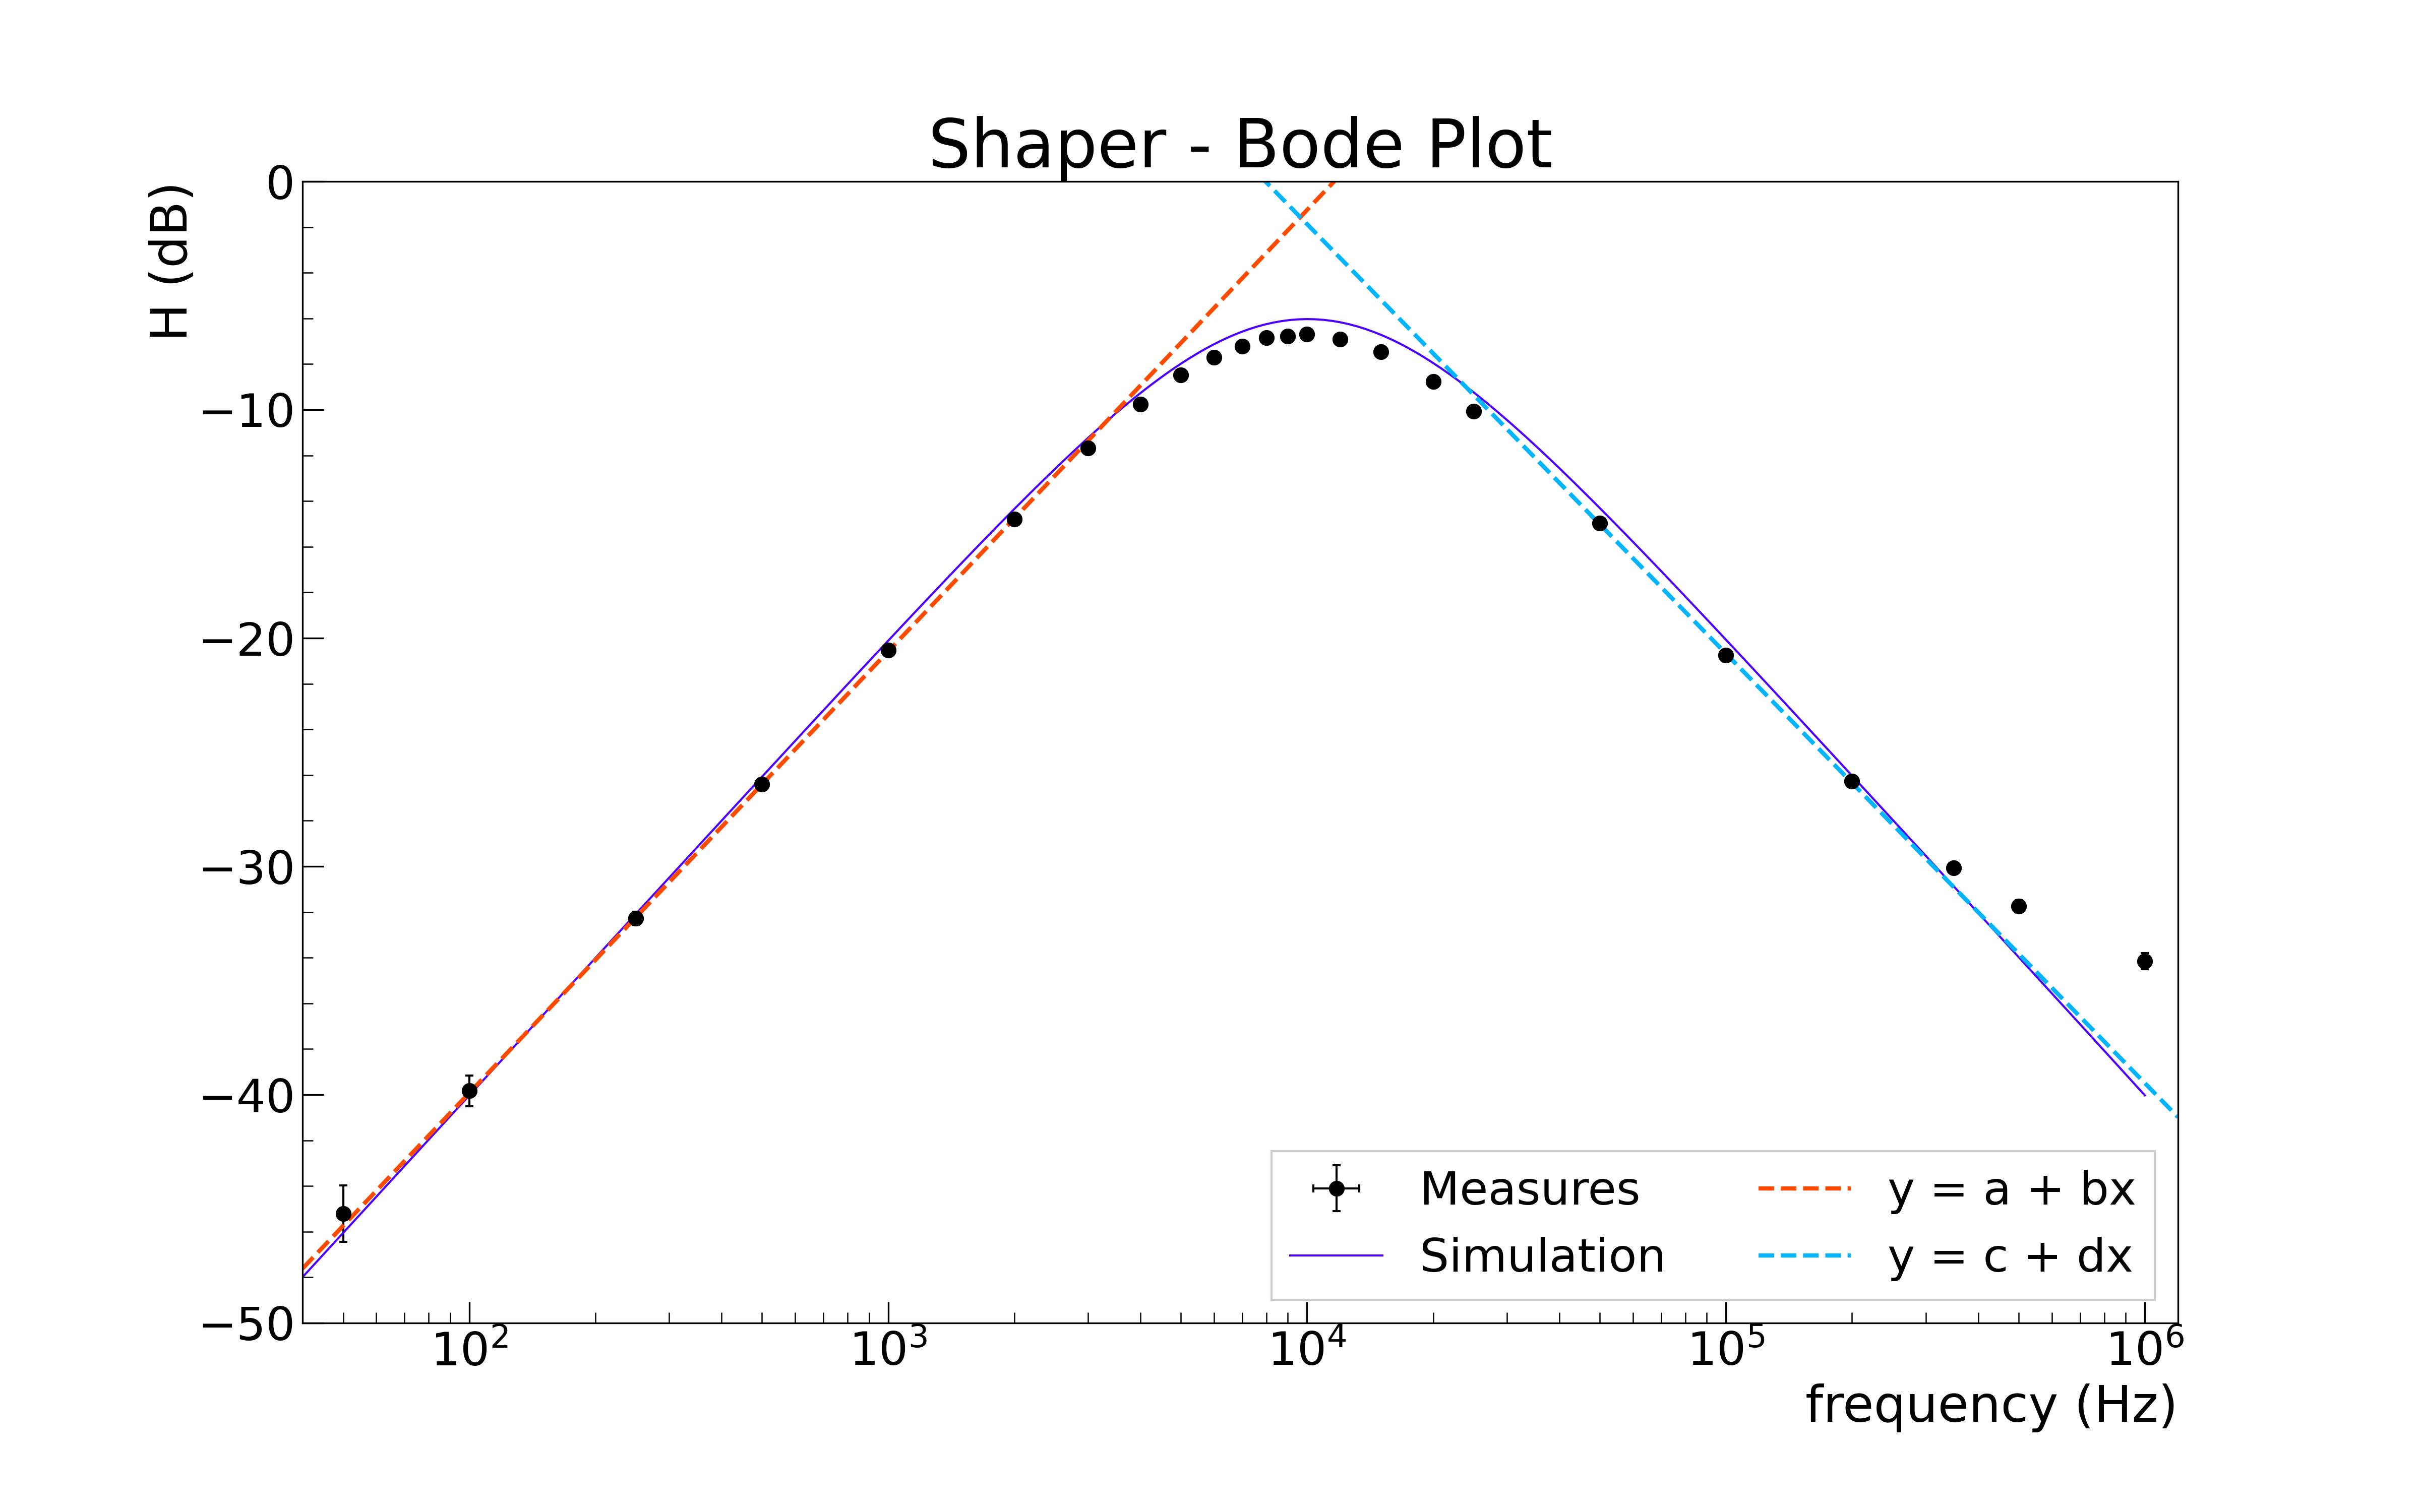
\includegraphics[width=0.9\linewidth]{../Plots/Shaper/bode_plot.png}
	\caption{\small Grafico di Bode delle misure sperimentali e dei dati simulati.}
	\label{i:shaper_thebode}
\end{figure}
\noindent  decrescita lineare ad alte frequenze (zona di integrazione) con pendenza $-18.8 \pm 0.3 \,\text{dB/dec}$.
L'ascissa del punto di intersezione delle due rette di regressione fornisce una stima della frequenza relativo al polo
$f_{\text{polo}} = 9.6 \pm 0.2 \,\si{k\Hz}$, in ottima compatibilità con la frequenza del polo teorica esposta in
\autoref{e:shaper_ft_th} ($\lambda = 0.8$). Partendo dalla stima ottenuta per $f_{\text{polo}}$, si ricerca il valore
massimo della funzione di trasferimento: sottraendo infine $3\,\text{dB}$ a tale massimo e cercando le ascisse di
intersezione con le due rette di regressione si riesce a determinare la larghezza di banda $\Delta f$ del filtro. Si
ottiene quindi la \textit{mid band} dello shaper, delimitata da
\begin{align}\label{e:shaper_bw}
	f_{\text{low}} &= 3.7 \pm 0.4 \,\si{k\Hz} &
	f_{\text{high}} &= 26.1 \pm 0.8\,\si{k\Hz}
\end{align}
\noindent Si vuole infine sottolineare che l'ottimo accordo della frequenza $f_{\text{polo}}$ con l'aspettativa teorica
(in cui compare la media pesata $\tau^{\text{sh}}$) supporta ulteriormente la validità dell'approssimazione
$\tau^{\text{sh}}_1 \approx \tau^{\text{sh}}_2$.

%-------------------------------------------------------------------------------------------------------------------------------------------
%	SHAPER + PREAMP
%-------------------------------------------------------------------------------------------------------------------------------------------

\subsection{Shaper con Preamplificatore in ingresso}\label{s:shaper_preamp}

In questa sezione si vuole studiare il comportamento dello shaper con in ingresso il segnale elaborato dal
preamplificatore. Il generatore di funzioni viene configurato nuovamente come in \autoref{s:preamp_config}: impulso
quadrato di frequenza $f_{\text{gen}} = 1 \,\si{k\Hz}$, tensione di riferimento $V_{\text{high}} = 0 \,\si{\volt}$,
ampiezza \textit{negativa} $V_{\text{low}} = -1 \,\si{\volt}$ e durata $T = 5 \,\si{\us}$. In questa configurazione, il
segnale in ingresso allo shaper corrisponde a quello rappresentato in \autoref{i:preamp_waveform}: la salita è ora
lineare, non più "istantanea", ed il segnale è smorzato esponenzialmente, non più costante al valore massimo. Questa
deviazione dall'idealità del segnale in ingresso allo shaper porta a rilevanti deformazioni del segnale in uscita:
osservando il grafico a sinistra in \autoref{i:shaper_waveforms} si nota chiaramente il fenomeno di \textit{undershoot}.
Il segnale, infatti, dopo aver raggiunto il massimo scende sotto allo zero (\textit{baseline}) per poi tendere ad esso
abbastanza lentamente (nel caso ideale dopo $200\,\si{\us}$ il segnale si è già azzerato, in questo caso invece è
necessario attendere circa $600\,\si{\us}$). La risoluzione di questo problema consiste nel porre una resistenza
adeguata in parallelo alla capacità $C_{1}$: scegliendo questa tale che $R_{\text{pz}} =
\frac{\tau^{\text{pre}}}{C_{1}}$, si trova $R_{\text{pz}} \gg R_{1}$ e di conseguena la funzione di trasferimento
\begin{align}
	H(s) &= 
		\frac{
			s + \frac{ 1 }{ \tau^{ \text{pz} } }
			}
			{
			s + \frac{ 1 }{ \tau^{ \parallel } }
			} 
		\approx
		\frac{
			s + \frac{ 1 }{ \tau^{ \text{pz} } }
			}
			{
			s + \frac{ 1 }{ \tau^{ \text{sh} } }
			} &
	&\text{con} \,\,\,\,	
	\begin{cases}
		\tau^{ \text{pz} } = C_{ 1 }\, R_{ \text{pz} }  \\
		\tau^{ \parallel } = C_{ 1 }\left(\frac{1}{R_{1}}+\frac{1}{R_{\text{pz}}}\right)^{-1}\\
	\end{cases}	
\end{align}
\noindent risulta, in buona approssimazione, avere lo stesso polo di 


\begin{figure}[H]
	\centering
	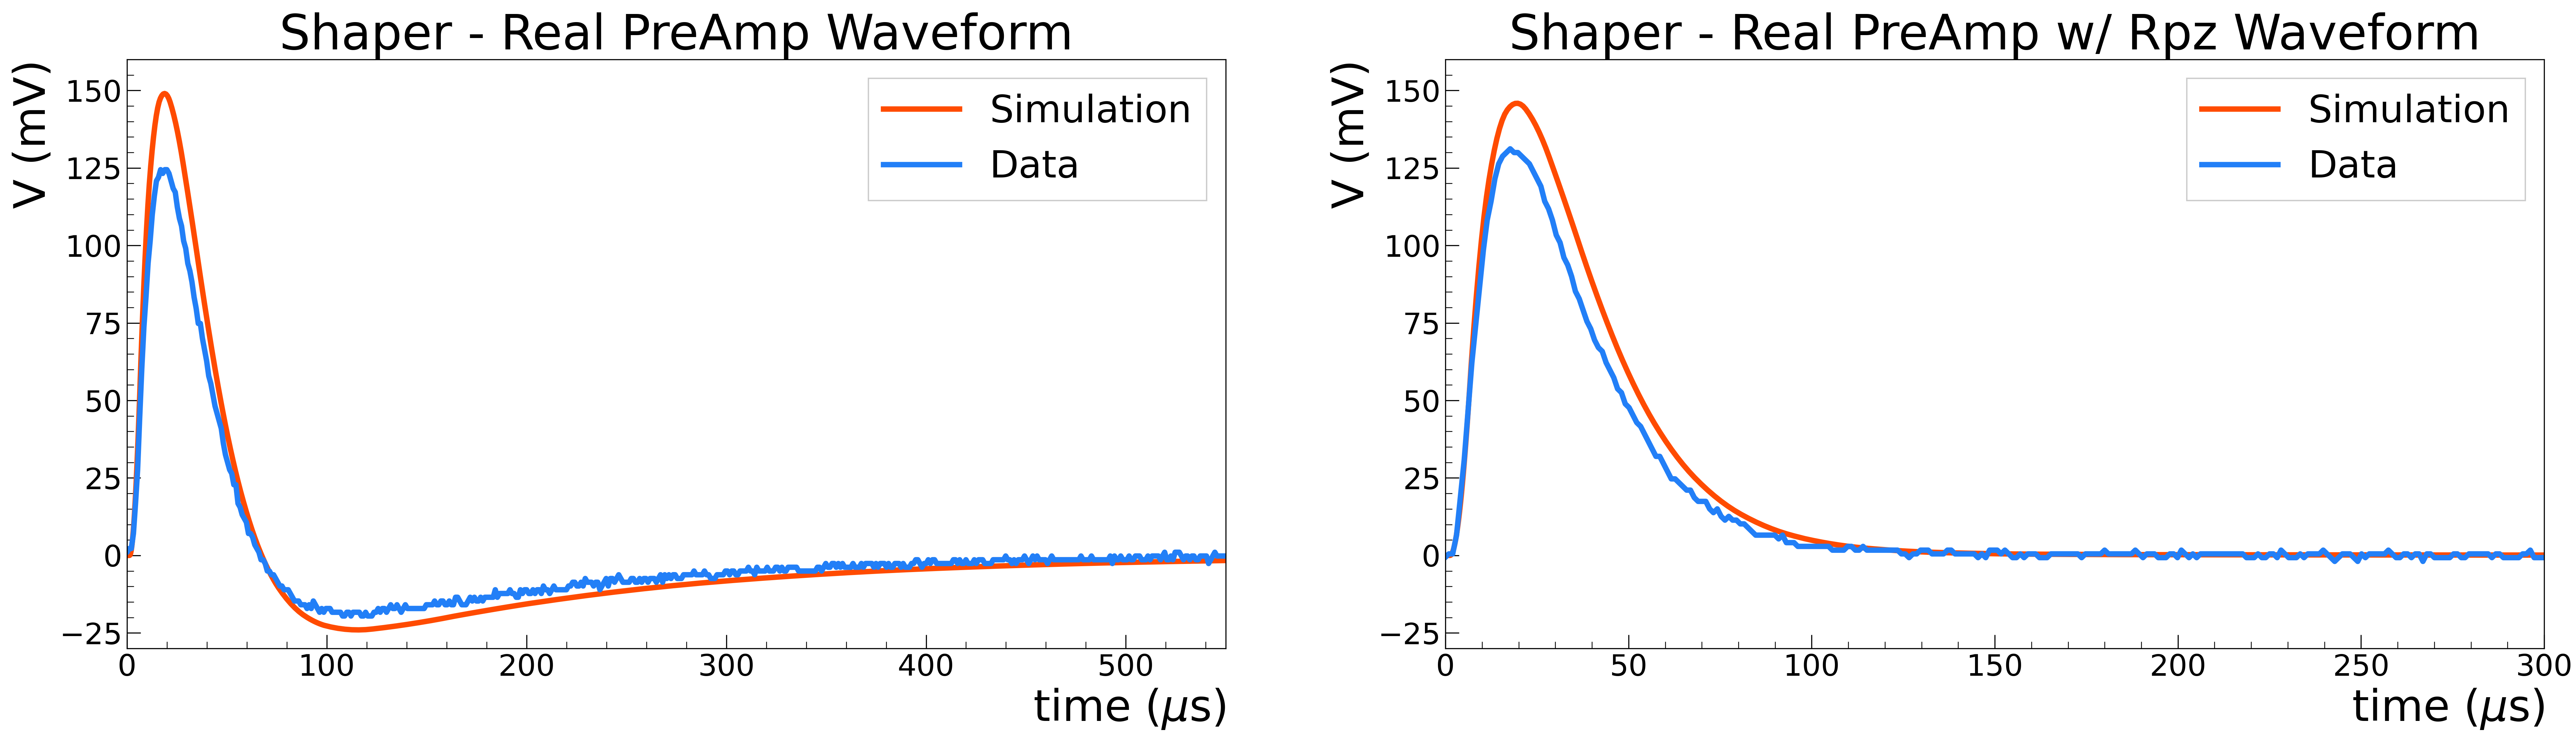
\includegraphics[width=\linewidth]{../Plots/Shaper/shaper_preamp_waveforms.png}
	\caption{\small A sinistra: segnale in uscita dallo shaper senza resistenza di compensazione. 
					A destra: segnale in uscita dallo shaper con resistenza di compensazione.}
	\label{i:shaper_waveforms}
\end{figure}












%----------------------------------------------------END OF FILE----------------------------------------------------------------------------
\end{document}